
\chapter{Региональная широкополосная грозопеленгационная система}
\label{sec:lds-intro}
Информация, собираемая грозопеленгационными системами, важна для решения задач оперативного мониторинга молниевой активности, краткосрочного прогноза быстроразвивающихся конвективных явлений, изучения климатологии молний и других прикладных и фундаментальных задач. Безопасность движения воздушных судов напрямую зависит от оперативной информации о молниевой активности, поскольку грозовые фронты являются помехами воздушному движению. Надежная молниезащита наземных объектов требует знания удельной поражаемости определенных территорий молниями, величин средних и максимальных токов разрядов, и других параметров. Зачастую грозы являются предвестниками развития опасных событий, таких, как шквал и катастрофические ливневые осадки, смерчи, град \cite{Matveev1984}. Например, быстрое увеличение числа внутриоблачных разрядов в единицу времени до 60~р/мин является признаком возникновения шквала или торнадо в течение 10-15 мин. Изменение преобладающей полярности молний с отрицательной на положительную является признаком начала формирования градовых частиц в облаке, а обратный процесс "--- об окончании градоопасной стадии \cite{Matveev1984}. С другой стороны, оперативные данные местоположения молний позволяют верифицировать прогнозные алгоритмы и реализовывать системы корректировки (<<nudging>>) численных моделей в соответствии с наблюдаемыми явлениями \cite{Huang2009}. 

Грозопеленгационные сети, совместно аэроэлектрическими наблюдениями \cite{Anisimov2013}, являются основой для задачи усвоения геоэлектрических метеоданных, исследований глобальной электрической цепи и климатологии молнии \cite{Mareev2010,Williams2014}. Статистика параметров молниевых разрядов напрямую связана с особенностями процессов, возникающих при инициации и развитии молнии, что позволяет развивать физику молниевого разряда. Совместное применение ГПС и других методов наблюдения за грозами порождает дополнительные возможности исследования окружающей природы.

Одним из путей развития мировой грозопеленгации является развертывание и совершенствование глобальных сетей местоопределения молниевых вспышек, основанных на приеме сверхдлинноволнового (СДВ) электромагнитного излучения. Лидирующие позиции в данном сегменте занимают сети WWLLN \cite{wwllnSite} и GLD360 \cite{gld360Site}. Однако, СДВ-системы обладают серьёзными недостатками: они регистрируют не более 20-30\% от общего числа вспышек облако-земля, имеют трудности с определением полярности молнии и не предоставляют информацию о внутриоблачных разрядах, что значительно затрудняет использование данных для оперативного мониторинга. Тем не менее, глобальные сети оказываются полезны для исследования климатологии молний, валидации глобальных и мезомасштабных прогнозов.

В настоящее время во всем мире активно развиваются региональные системы, позволяющие с высокой точностью фиксировать как разряды типа облако-земля, так и внутриоблачные разряды, и определять большое количество параметров вспышек \cite{Pinto2003,nldnSiteArticle}.

В данной главе приведён обзор существующих грозопеленгационных систем, а также описана разработанная автором регональная грозопеленгационная система OpenLDS \cite{BulatovMiG}. Система введена в эксплуатацию в течение конвективного сезона 2014 г. и работает в непрерывном режиме. Нижегородская ГПС является многопунктовой. Приёмники системы  работают в СДВ и ДВ-диапазоне. К конвективному сезону 2017~г. ГПС расширена до 6 пунктов пеленгации и покрывает область размерами порядка 1500~км. Проведена оценка точности разработанной системы на основании сравнения с данными международной ГПС WWLLN и показаниями ДМРЛ, установленного в Нижнем Новгороде. На основе показаний ГПС исследовано распределение гроз в регионе. Исследованы статистические особенности мультипликативности обратного удара и максимальных токов повторных разрядов.

\section{Классификация грозопеленгационных систем}
Грозопеленгационная система (ГПС) представляет собой ап\-па\-рат\-но-про\-грамм\-ный комплекс, предназначенный для определения положения молниевых разрядов в пространстве, времени их возникновения, а также их характеристик. Грозопеленгационные системы можно классифицировать по следующим признакам:
\begin{itemize}
	\item \textbf{Распределённость.} Однопунктовые системы содержат только одно устройство регистрации электромагнитного излучения (грозопеленгатор), а многопунктовые включают в себя несколько грозопеленгаторов, распределенных на некоторой площади. При этом данные, получаемые с разных грозопеленгаторов, обрабатываются совместно. Многопунктовые грозопеленгационные системы также называют грозопеленгационными сетями. Такие системы обладают большей точностью и надёжностью, однако их разработка сложнее, а стоимость развёртывания "--- больше.
	\item \textbf{Частотный диапазон.} Определяется диапазоном при\-ем\-ни\-ков-гро\-зо\-пе\-лен\-га\-то\-ров, используемых в системе. Широкое распространение имеют ГПС, работающие в СДВ-диапазоне. Приемники таких систем способны регистрировать разряды со всего земного шара (при достаточной чувствительности). Также, распространены ГПС, работающие в ДВ, КВ и УКВ диапазонах. 
	\item \textbf{Метод пеленгации.} Для определения положения молнии многопунктовыми ГПС наиболее часто применяются метод пересечения пеленгов (direction finding), разностно-дальномерный метод (time-of-arrival), а также их комбинации и модификации. Однопунктовые ГПС определяют пеленг молнии по горизонтальным компонентам магнитного поля, а расстояние "--- по разности фаз между магнитным и электрическим полем, интенсивности и другим параметрам сигнала.
	\item \textbf{Доступность данных.} Результаты работы ГПС могут быть доступны или недоступны для внешних исследователей. Доступ может осуществляться на платной, либо бесплатной основе с теми или иными ограничениями. Системы, ориентированные на финдаментальные исследования, предоставляют доступ к архиву данных за продолжительный срок, в то время как системы, ориентированные на оперативный мониторинг предоставляют данные с наименьшей задердкой. Также, имеет значение доступность первичных данных грозопеленгации: записей электромагнитных полей и временных меток приёмников. 
	\item \textbf{Открытость алгоритмов работы.} Большинство систем грозопеленгации не раскрывают деталей алгоритмов позиционирования разрядов, что затрудняет анализ данных.
\end{itemize}

Применительно к задачам грозопеленгации, выделяют следующие характеристики молниевых разрядов:
\begin{itemize}
	\item Тип разряда "--- внутриоблачный, либо облако-земля
	\item Знак заряда, переносимого из облака на землю "--- положительный, либо отрицательный
	\item Максимальный и средний токи молнии
	\item Величина перенесенного заряда
	\item Количество повторных обратных ударов
\end{itemize}
и другие характеристики. Устройство, предназначенное для регистрации в той или иной форме электромагнитного излучения молний называют грозопеленгатором.

\section{Существующие системы грозопеленгации}
\label{sec:lds-review}
На данный момент в мире функционирует несколько глобальных грозопеленгационных систем, охватывающих весь земной шар, и значительное число региональных, области покрытия которых имеют характерный размер от сотен до десятков тысяч километров. На территории России также развернуто несколько ГПС, отличающихся параметрами и назначением.

\subsection{Зарубежные и международные ГПС}
Рассмотрим особенности и характеристики наиболее значимых грозопеленгационных систем, разрабатываемых и поддерживаемых зарубежными коллегами.
% Информация здесь: https://link.springer.com/article/10.1007/s10712-013-9251-1#Sec18

\subsubsection{World Wide Lightning Location Network}
Грозопеленгационная система World Wide Lightning Location Network\cite{wwllnSite} (WWLLN, принятое русское произношение <<Вулин>>) "--- глобальная ГПС, поддерживаемая Университетом Вашингтона, Сиэтл. Основное назначение системы "--- научные исследования. Доступны данные с 15~августа~2014~года.

Система WWLLN объединяет более 70~грозопелегаторов по всему миру и работает в СДВ-диапазоне, 3--30\,КГц. Поскольку пеленгаторы находятся на достаточно большом удалении друг от друга, WWLLN обнаруживает только наиболее интенсивные молнии. Согласно \cite{wwllnSite}, только 15--30\%~разрядов, зарегистрированных одним грозопеленгатором, регистрируются не менее чем 4~другими. Для вспышек с пиковым током более~30\,кА регистрируется около 30\%~событий.

Для определения положений молниевых разрядов системой WWLLN применяется метод time of group arrival (<<TOGA>>) "--- разновидность разностно-дальномерного метода с модификациями, являющимися коммерческой тайной WWLLN.

На основе сравнения показаний системы WWLLN и системы OpenLDS, созданной в рамках данной работы, на территории Нижегородской области погрешность позиционирования разрядов WWLLN составляет, приблизительно, 4\,км с систематическим смещением с систематическим смещением 2,2\,км на северо-запад\cite{BulatovMiG}.

Важной аппаратной особенностью WWLLN, существенно ограничивающей её возможности, является применение звуковых карт персональных компьютеров в качестве АЦП пунктов грозопеленгации.

\subsubsection{U.\,S. National Lightning Detection Network}
U.\,S. National Lightning Detection Network\cite{nldnSiteArticle} (NLDN) "--- грозопеленгационная система, разработанная компанией Vaisala по заказу правительства США.

Система NLDN обладает высокой точностью на территории США и состоит из более чем 100~пунктов пеленгации, расположенных сеткой с характерным шагом 300--350\,км. Диапазон работы приёмников составляет 400\,Гц--400\,кГц. Регистрируются как разряды облако-земля, так и внутриоблачные. Максимальные токи молний определяются при помощи эмпирической формулы, основанной на данных триггерных молний. Согласно исследованию \cite{Biagi2007}, на территории Южной Аризоны NLDN регистрирует 76\% молний, а в Оклахоме, штат Техас "--- 85\%. \cite{Rakov-emld}

Для определения положения молний применяется комбинация разностно-дальномерного метода и метода пересечения пеленгов \cite{Rakov-emld}. Алгоритмы обработки данных системой NLDN закрыты и являются коммерческой тайной. 

\subsubsection{Global Lightning Dataset }
Global Lightning Dataset (GLD360), также называемая Global Lightning Detection Network (GLDN) "--- глобальная система СДВ-диапазона разработки компании Vaisala. 

Согласно \cite{Demetriades2010}, эффективность детектирования молний системой GLD360 на территории США составляет 86–92\% при средней ошибке позиционирования 10,8\,км. Однако согласно \cite{Naccarato2010}, на территории Бразилии система регистрирует около 16\% вспышек с ошибкой 12,5\,км. Помимо координат, система определяет максимальные токи и полярность молний, основываясь на записях электромагнитного поля. Определение типа разряда происходит посредством сравнения с известными <<каноническими>> сигналами. \cite{Rakov-emld}

Позиционирование молний происходит с использованием комбинации разностно-дальномерного метода и метода пересечения пеленгов \cite{Rakov-emld}. Данные GLD360 доступны по платной подписке. Алгоритмы работы системы не раскрываются.

\subsubsection{Earth Networks Total Lightning Network}
Система Earth Networks Total Lightning Network (ENTLN) действует на территории США и ряда другиз стран \cite{Rakov-emld}. Система работает в широкой полосе частот от 1\,Гц до 12\,МГц. Применяется разностно-дальномерный метод пеленгации. Сигнал с электрической антенны используется как для определения положения молний, так и для разделения разрядов по типу: внутриоблачные или облако-земля. Разряды удаленные не более, чем на 10\,км и отстоящие по времени не более, чем 700\, считаются относящимися к одной молнии. \cite{Heckman2010}

По заявлениям разработчиков \cite{Heckman2010}, система регистрирует 40--50\% внутриоблачных разрядов на большей части территории США и до 95\% на среднем западе и востоке США. Высокая чувствительность к внутриоблачным разрядам является приоритетом ENTLN.

\subsection{Отечественные ГПС и исследования на их основе}
Обзор основных результатов российских исследователей в области грозопеленгации на 2015\,г. представлен в обзоре\cite{MareevWe2016}.

На территории нашей страны также развиваются системы многопунктовой грозопеленгации. Проводятся работы по исследованию и улучшению показателей точности существующих систем \cite{Kononov2014,Kononov2013}, разрабатываются новые системы и комплексы \cite{Adjiev2013,BulatovMiG}. Проводятся исследования, использующие данные грозопеленгации отдельно, а также совместно с другими источниками информации о молниевой активности \cite{Buharov2013}.

На территории Северного Кавказа впервые в России введен в эксплуатацию грозорегистратор LS 8000 фирмы «Vaisala». Он обеспечивает определение координат, полярности, типа (облако-облако или облако-земля), токов и других характеристик молниевых разрядов. Предполагается совместная кластерная обработка данных LS 8000 с картой радиоэха облаков и осадков, полученной региональной сетью МРЛ в реальном времени. За период эксплуатации грозорегистратора LS 8000 с 2008 г. проведены исследования параметров токов зарегистрированных разрядов облако-земля. \cite{Adjiev2013} 

В течение 2011 г. модифицирована грозопеленгационная система <<Алвес 9.07>>\cite{AlwesSite}, разработанная ООО <<Алвес>>, совместно с сотрудниками отдела Атмосферного электричества Главной геофизической обсерватории. Система <<Алвес>> основанная на разностно-дальномерном принципе и покрывает территорию Европейской части России и Урал. Разработано и внедрено новое поколение грозорегистраторов. По данным на август 2014 г. в состав системы входят 70 разнесенных пунктов регистрации гроз. В течение конвективных сезонов 2013-2014 гг. проведены оценки точностных характеристик сети с использованием данных локации грозовых очагов европейской разностно-дальномерной сети Blitzortung \cite{Snegurov2010, AlwesSite}. Также, исследованы источники ошибок, обусловленные погрешностями временной привязки к сигналам атмосфериков в разнесенных пунктах системы. Произведены модельные и экспериментальные оценки величин этих погрешностей \cite{Kononov2011, Kononov2014}. Проведены модельные оценки погрешностей алгоритмов однопунктового определения координат сильноточного молниевого разряда в рамках его модели в виде произвольно ориентированного электрического диполя, обусловленных влиянием внешних атмосферных и индустриальных помех \cite{Kononov2013}.

На востоке Сибири исследованы особенности пространственного распределения положительных грозовых разрядов за 2003-2007 гг., зафиксированных однопунктовым грозопеленгатором-дальномером с радиусом наблюдения около 1200 км. Зафиксировано, что распределения положительных разрядов в целом отражают общую картину грозовой активности. Выделены области очагов грозовой активности, в которых отношение потока положительных разрядов к потоку отрицательных может превышать 1, что обусловлено географическими условиями — высокогорной местностью и близостью Охотского моря. Таким образом показано влияние рельефа местности на инвертирование расположения заряда в облаке \cite{Mullayarov2009}.

Проводятся исследования статистических характеристик электрических полей грозовых облаков на основе показаний флюксметров \cite{Our2013} в европейской части России. Получаемые данные могут быть сопоставлены показаниям региональной грозопеленгационной системы.

Исследованы прочие параметры молниевой активности на территории центральной Якутии в 2009-2012\,гг. Доля разрядов облако-земля определена, как 40-60\%, что соответствует наблюдениям в Западной Сибири (40-50\%). Количество положительных разрядов в землю составило 8-15\%. Грозовая активность в г. Якутске в 3 раза выше, чем в зоне радиусом 400 км вокруг Якутска, что свидетельствует о наличии т.\,н. <<городского эффекта>> (<<урбан-эффекта>>). \cite{Kozlov2014}

Также, в Якутии продолжительное время функционирует система, состоящая из трех однопунктовых грозопеленгаторов в городах Якутск, Нерюнгри, Мирный. Грозопеленгаторы работают в диапазоне СДВ и обладают точностью определения положения в несколько километров. На основе показаний системы совершенствуются алгоритмы кластеризации грозовых ячеек в кластеры. Результаты обработки данных показывают, что зрелые грозовые ячейки находятся в центре кластера, а диссипирующие "--- с подветренной стороны кластера. Время активности отдельной ячейки составляет 20-30 мин., а сам многоячеистый кластер может существовать несколько часов. Интенсивность грозы в кластере обычно выше, чем в изолированных грозовых ячейках. По результатам исследования 227 грозовых ячеек средняя площадь ячейки составляет 12\,$\text{км}^2$, среднее время существования "--- 31 мин, среднее число грозовых разрядов в ячейке "--- 10. Получены первые данные о климатологии гроз в регионе. \cite{Shabaganova2012}

\section{Постановка и решение задачи многопунктовой грозопеленгации}
\label{sec:lds-tasks}
Основной задачей ГПС является определение метоположения и времени возникновения молниевых разрядов. Рассмотрим общую постановку такой задачи и способы её решения.

Многопунктовая ГПС состоит из нескольких разнесенных пунктов грозопеленгации. Такие пункты оснащены магнитными и электрическими антеннами, а также точными часами, основанными на сигналах GPS. По точным часам аппаратным образом определяется момент прихода фронта электромагнитного импульса молниевого разряда в полосе работы приемника-грозопеленгатора. Данные со всех приёмников совместно обрабатываются процессинговым сервером. За счет корреляционной обработки записей электромагнитных полей временные отметки разных приёмников уточняются.

При возникновении молниевого разряда в радиусе чувствительности некоторого грозопеленгатора регистрируется следующая информация:
\begin{itemize}
	\item $P_i$ "--- GPS-координаты приёмника на поверхности Земли, его широта и долгота
	\item $t_i$ "--- момент прихода электромагнитного импульса. Определяется срабатывание триггера по превышению элекрическим и/или магнитным полем определенного порога
	\item $B^x_i(t), B^y_i(t), E^z_i(t)$ "--- записи горизонтальных компонент магнитного поля и вертикальной компоненты электрического. Не являются необходимыми для регения задачи пеленгации, однако позволяют повысить точность позиционирования
\end{itemize}

\subsection{Пространственно-временная кластеризация}
\label{sec:space-time-cluster}
Записи $\xi_i = \{P_i, t_i, B^x_i(t), B^y_i(t), E^z_i(t)\}$ от всех пеленгаторов для всех зарегистрированных разрядов поступают на сервер. В качестве первого этапа обработки данных, необходимо провести их пространственно-временную кластеризацию. Записи, которые \textit{могут} относиться к одному и тому же разряду, объединим в множества $C_j$, которые и назовём пространственно-временными кластерами. Поскольку такие записи обусловлены одной и той же причиной "--- разрядом, волна от которого распространяется со скоростью света, между событиями регистрации должен быть времени-подобный интервал, то есть для любых двух элементов кластера $i, j$ должно выполняться соотношение
\begin{equation}
	\frac{\rho(P_i, P_j)}{c} > (1+\varepsilon) |t_i - t_j|.
\end{equation}
где $\rho(P_i, P_j)$ "--- расстояние на поверхности Земли между точками $P_i$ и~$P_j$, $\varepsilon$ "--- поправка для учёта погрешности определения координат и времени.

После такой процедуры все записи группируются в пространственно-временные кластеры $C_j = \{\xi^j_1, \ldots, \xi^j_{N_j}\}$. Для каждого кластера независимо решается задача пеленгации: нахождение координат разряда $X_j(C_j)$ и времени его возникновения $T_j(C_j)$. Также, если кластер не обусловлен реальным разрядом, а образовался вледствие погрешности измерений или антропогенных шумов, должен быть предусмотрен механизм его отбраковки.

Заметим, что при успешном нахождении $X_j(C_j)$, задача нахождения $T_j(C_j)$ является тривиальной. Для каждого пеленгатора, запись которого есть в кластере $C_j$ нужно посчитать время, за которое до него дошел электромагнитный имульс из известной точки $X_j$, и вычесть из времени регистрации импульса этим пеленгатором. Полученные величины усреднить по всем записям в кластере для увеличения точности:
\begin{equation}
	T_j(C_j) = \frac{1}{N_j} \sum_{i=1}^{N_j} \left( t^j_i - \frac{\rho(X_j, P^j_i)}{c} \right),
\end{equation}
где $t^j_i, P^j_i \in \xi_i^j \in C^j$.

Рассмотрим далее основные методы определения положения разряда. Поскольку все исходные данные известны с определенной погрешностью, задача определения $X_j(C_j)$ будет сведена к задаче минимизации некоторой функции ошибки $\Psi(X, C_j)$, зависящей от положения разряда и всех данных в кластере $C_j$:
\begin{equation}
	X_j = X~|~\Psi(X, C_j) \rightarrow \min
\end{equation}

Таким образом, положением разряда будет считаться наиболее подходящее положение с точки зрения некоторого алгоритма пеленгации. Оптимизационный подход также позволяет комбинировать несколько методов позиционирования разряда:
\begin{equation}
	\Psi(X) = \alpha_1 \Psi_1(X) + \ldots + \alpha_N \Psi_N(X),
	\label{eq:errfunc-combo}
\end{equation}
где $\Psi_{i}(X)$ и $\alpha_i$ "--- функция ошибки и коэффициент доверия для метода $i$.

\subsection{Метод пересечения пеленгов}
Если каждый грозопеленгатор оснащен скрещенными магнитными антеннами, регистрирующими горизонтальные компоненты магнитного поля, возможно восстановить усредненное направление магнитного поля. Записи $B^x_i(t), B^y_i(t)$ представляют собой дискретные ряды данных, которые можно изобразить на плоскости $(B^x, B^y)$ в виде точек, как показано на рисунке TODO. Методом линейной регрессии выделяется направление $\vec{l_i}$, вдоль коротого колеблется поле. При этом $\vec{l_i}$ определен с точность до знака.

При условии, что приёмник находится в дальней зоне излучения молниевого разряда, можно считать, что направление на источник электромагнитного поля и вектор $\vec{B}$ перпендикулярны. Таким образом, для каждой записи можно определить азимут разряда $\varphi_i$. Однако, поскольку $\vec{l_i}$ определен с точность до знака, $\varphi_i$ определен с точностью до поворота 90 градусов.

Зная $\varphi_i$ для каждой записи в некотором кластере $C^j$, можно составить функцию потерь метода пересечения пеленгов, как
\begin{equation}
	\Psi_{df}(X, C^j) = \sum_{i=1}^{N_j} (\delta(\varphi_i, \varphi(P_i, X)))^2,
\end{equation}
где $\varphi(P_i, X)$ "--- азимут направления между точками $X$ и $P_i$ на интервале $[-180\degree, 180\degree]$, а $\delta(\varphi_1, \varphi_2)$ "--- минимальный угол между направлениями $\varphi_1, \varphi_2$.

Преимуществом метода пересечения пеленгов является возможность работы при наличии всего двух грозопеленгаторов: При ограниченном радиусе действия приёмников пересечение двух прямых на поверхности Земли единственным образом определяет источник сигнала.

Недостатком метода является относительно низкая точность определения положения разрядов. Погрешность позиционирования линейно возрастает с удалением от ближайших приёмников. Метод чувствителен к точности ориентировки магнитных антенн по осям север-юг и восток-запад. Отклонение плоскости антенны всего на 5\textdegree ~приводит к отклонению пеленга на 2,7\,км при удалении в 100\,км от приёмника. При реальной эксплуатации системы ГПС ориентировка антенны с ошибкой менее 10\textdegree~зачастую невозможна.

\subsection{Разностно-дальномерный метод}
Альтернативой методу пересечения пеленгов является разностно-дальномерный метод. Зная для кластера $C_j$ точные моменты $T_i^j$ регистрации электромагнитного импульса молнии пеленгаторами с координатами $P_i^j$, запишем разность времени прихода импульса для пробной точки:
\begin{equation}
	\Delta T(X, P_l^j, P_k^j) = \frac{\rho(X, P_l^j) - \rho(X, P_k^j)}{c}.
\end{equation}
Поскольку реально измеренная разность времени прихода импульса известна и составляет $T_l^j - T_k^j$, квадраты величин $\Delta T$ можно просуммировать для всех пар грозопеленгаторов из кластера $C_j$, и функция ошибки разностно-дальномерного метода может быть записана следующим образом:
\begin{equation}
	\Psi_{ta}(X, C^j) = \sum_{k=1}^{N_j} \sum_{l=1, l \ne k}^{N_j} \left( \frac{\rho(X, P_l^j) - \rho(X, P_k^j)}{c} - (T_l^j - T_k^j)\right)^2.
\end{equation}

Преимуществом данного метода являются минимальные требования к приёмникам-грозопеленгаторам, а также относительно высокая точность. Приёмники должны лишь точно регистрировать момент времени прихода импульса, в то время как запись электромагнитных полей не требуется. Достаточно одного канала приёма со штыревой вертикальной электрической антенны. Также, необходимо однократно определить координаты грозопеленгатора.

\subsection{Решение задачи пеленгации}
Для нахождения координат и времени молниевого разряда для каждого необходимо решить задачу оптимизации функции ошибки~\eqref{eq:errfunc-combo}. Для решения данной задачи применяется градиентный спуск из множества начальных точек, равномерно распределенных по площади действия ГПС.

В результате проведенного исследования точности системы (см.~п.\,\ref{sec:lds-valid}) было установлено, что разностно-дальномерный метод существенно превосходит в точности метод пересечения пеленгов, а также комбинацию обоих этих методов. Данное утверждение не является универсальным, однако справедливо для использованного в работе оборудования и условий его эксплуатации.

\section{Устройство грозопеленгационной системы}
\label{sec:lds-inside}
Разработанная система грозопеленгации состоит из автономных пунктов пеленгации, сервера базы данных и процессингового сервера. Пункты грозопеленгации производят автоматическое наблюдение электромагнитного излучения молниевых разрядов и временное хранение результатов наблюдения до передачи на сервер базы данных. Они расположены сеткой на территории исследуемого района на расстоянии 50-200 км. Для работы системы в заданном районе необходимо не менее двух пунктов пеленгации. Сервер базы данных грозопеленгационной сети аккумулирует результаты наблюдения электромагнитных полей, собранные пунктами грозопеленгации, а также хранит результаты обработки данных: положения и характеристики молниевых разрядов. Процессинговый сервер определяет местоположения и характеристики молниевого разряда, анализируя данные наблюдений электромагнитных полей. Также процессинговый сервер содержит пользовательский веб-интерфейс, позволяющий удаленно работать с грозопеленгационной сетью с любого компьютера, подключенного к сети Internet. Общая организация системы представлена на \figRef{fig:lds-schematic}.

\begin{figure}[h]
	\center{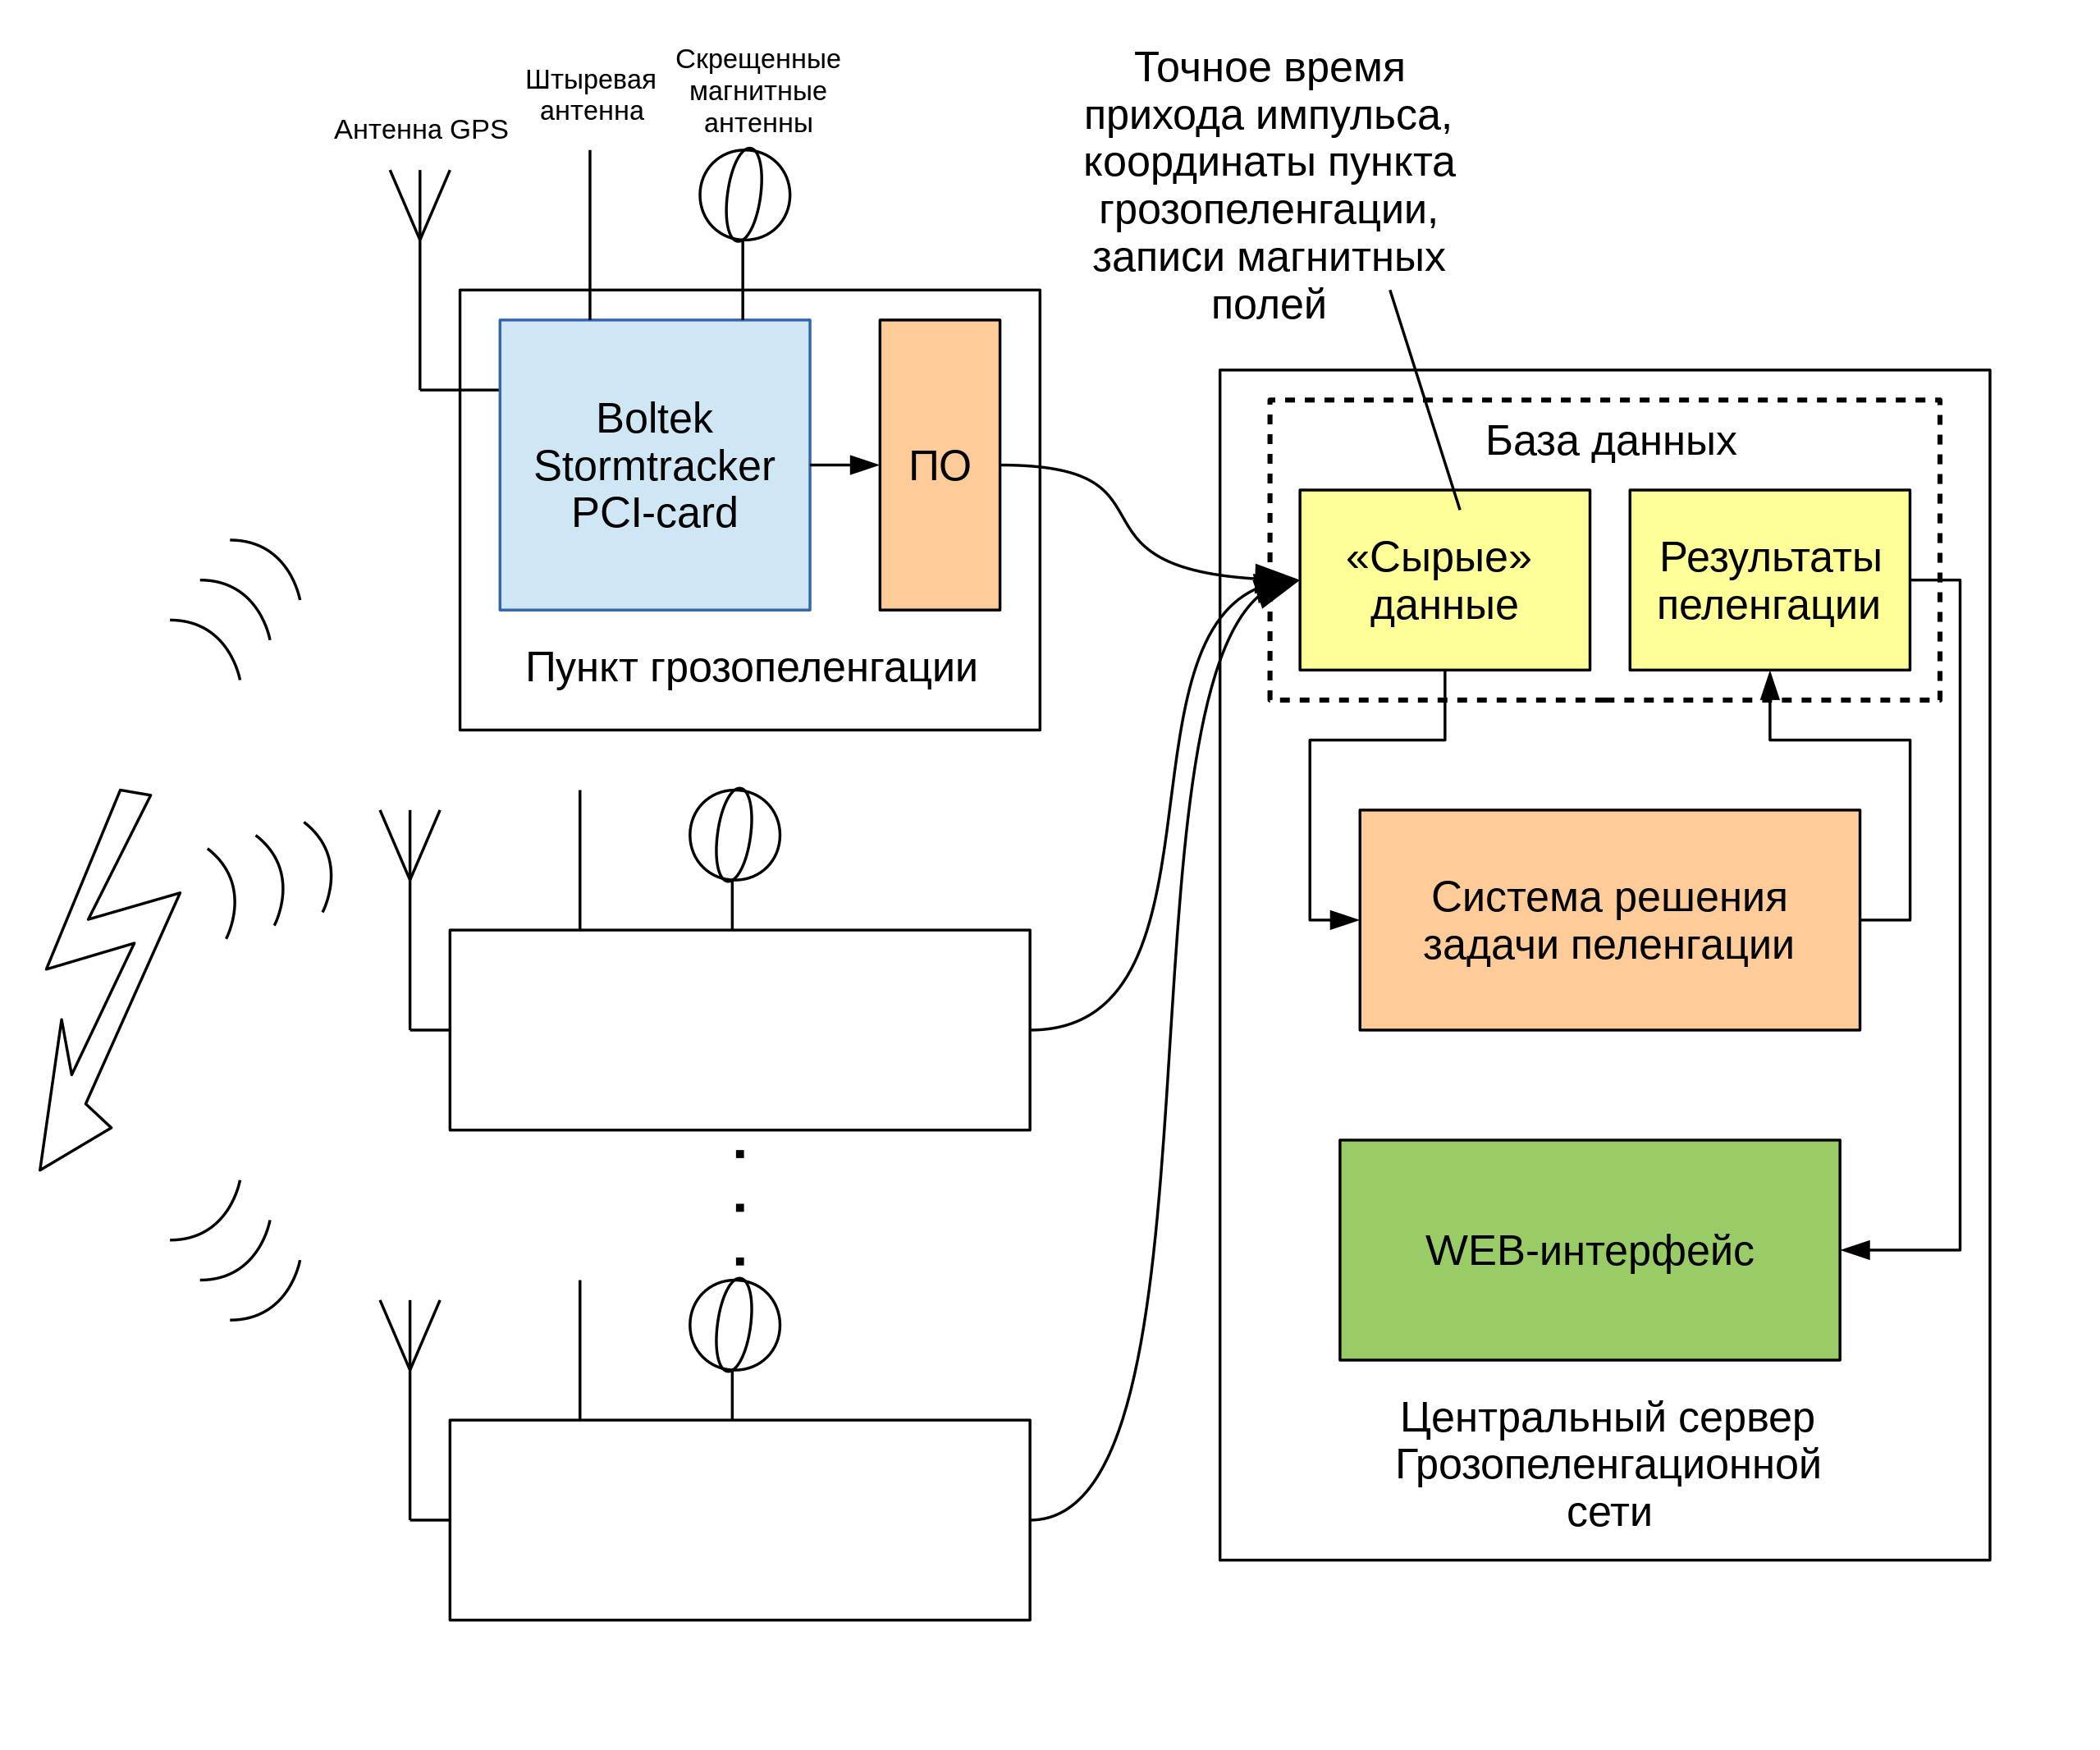
\includegraphics[width=\linewidth]{lds-schematic.png}}
	\caption{Организация грозопеленгационной системы}
	\label{fig:lds-schematic}
\end{figure}

Пункт грозопеленгации включает в себя персональный компьютер, оснащенный PCI-картой Boltek Stormtracker и модулем расширения Boltek LTS2. К PCI-карте подключены антенное устройство в виде двух скрещенных магнитных антенн, принимающих ортогональные горизонтальные компоненты магнитного поля и штыревой электрической антенны, а также GPS-модуль для точного измерения времени прихода электромагнитного импульса, создаваемого молнией. Компьютер оснащен специально разработанным программным обеспечением, работающим под операционной системой GNU/Linux, обеспечивающим сбор, временное хранение и пересылку результатов наблюдения электромагнитных полей на сервер базы данных. Передача данных осуществляется по сети Internet. Технические характеристики пункта грозопеленгаци приведены в таблице~\ref{tab:lds-pars}.

\begin{table}[h]
	\begin{center}
		\begin{tabular}{l|l}
			Характеристика & Значение \\
			\hline
			Частотный диапазон приёмника & $15\ldots100$\,КГц \\
			Частота дискретизации АЦП & 8\,МГц \\
			Разрядность АЦП & 8\,бит \\
			Размер буфера АЦП & 64\,мкс \\
			Минимальный интервал между регистрируемыми событиями & 400\,мкс \\
			Радиус покрытия пункта пеленгации & 400\,км \\
		\end{tabular}	
	\end{center}
	\caption{Характеристики пункта грозопеленгации на основе устройства Boltek Stormtracker}
	\label{tab:lds-pars}
\end{table}

Сервер базы данных грозопеленгационной сети представляет собой компьютер, подключенный к сети Internet, работающий под ОС GNU/Linux. На нём установлено программное обеспечение MariaDB для организации реляционной базы данных (БД) MySQL. База данных содержит в себе всю первичную информацию, поступающую от пунктов грозопеленгации, а также результаты решения задачи пеленгации \cite{rcpl2014}. Данный сервер также содержит веб-интерфейс для доступа к результатам работы системы. Интерфейс ГПС представлен на \figRef{fig:lds-web-interface}.

Решение задачи грозопеленгации происходит на отдельном процессинговом сервере, подключенном к серверу базы данных. Первичные данные загружаются из БД, выделяются пространственно-временные кластеры по алгоритму, описанному в п.\,\ref{sec:space-time-cluster}. Затем, минимизируется функция ошибки. Используемый метод определяется настройками~ПО. Результаты кластеризации, а также точное время и положение молниевого разряда записываются в~БД.

\begin{figure}[h]
	\center{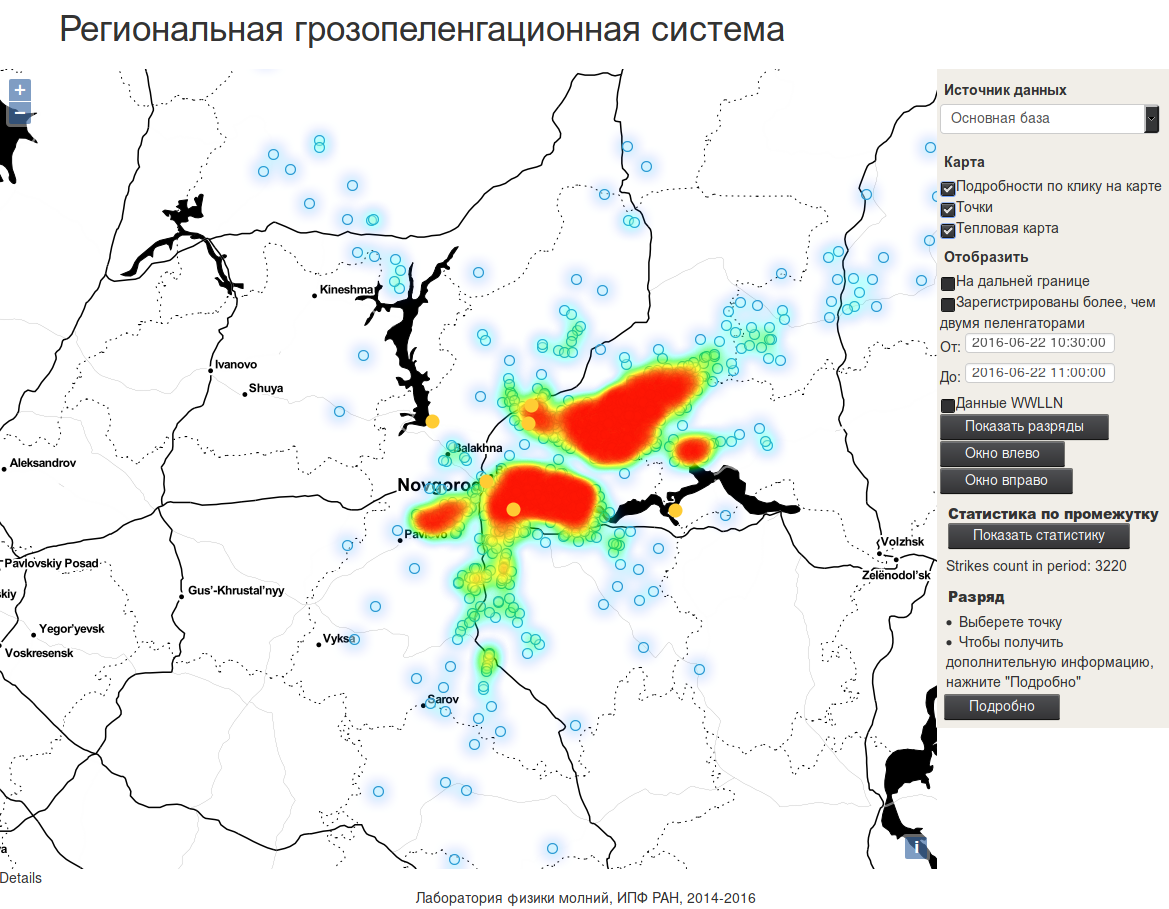
\includegraphics[width=0.9\linewidth]{lds-web-interface.png}}
	\caption{Веб-интерфейс грозопеленгационной системы}
	\label{fig:lds-web-interface}
\end{figure}

Программное обеспечение грозопеленгационной системы разработано в рамках данной работы в соответствии с требованиями к отказоустойчивости, расширяемости и гибкости. При пропадании интернет-соединения между грозопелнегаторами и сервером базы данных информация не теряется, и при восстановлении соединения в целости передаётся в БД. Перемещение пункта пеленгации не требует перенастройки ПО, таким образом системой поддерживаются мобильные грозопеленгаторы. Для добавления нового пункта необходимо лишь добавить одну запись в таблицу конфигурации.

В настоящее время автором данной работы ведётся разработка собственного аппаратного обеспечения для грозопеленгаторов, что позволит существенно снизить стоимость оборудования, габариты приёмников и их энергопотребление. Вследствие этого будет увеличена плотность покрытия~ГПС. В основе будущего грозопеленгатора лежит микроконтроллер STM32F407, подключаемый к одноплатному компьютеру через интерфейс~USB. На данный момент разработаны схемы, встраиваемое программное обеспечение и печатные платы устройства.

\section{Пример работы ГПС}
\label{sec:lds-example}

Для демонстрации возможностей региональный грозопеленгационной системы, как инструмента исследования молниевой активности, рассмотрим грозу 16 июля 2016 г, проходившую на территории Нижегородской области с 14:50 по 16:30 GMT. Она прошла с запада на восток со скоростью в среднем 18 км/ч от г.~Заволжье до ст.~Линда.

\begin{figure}[h]
	\center{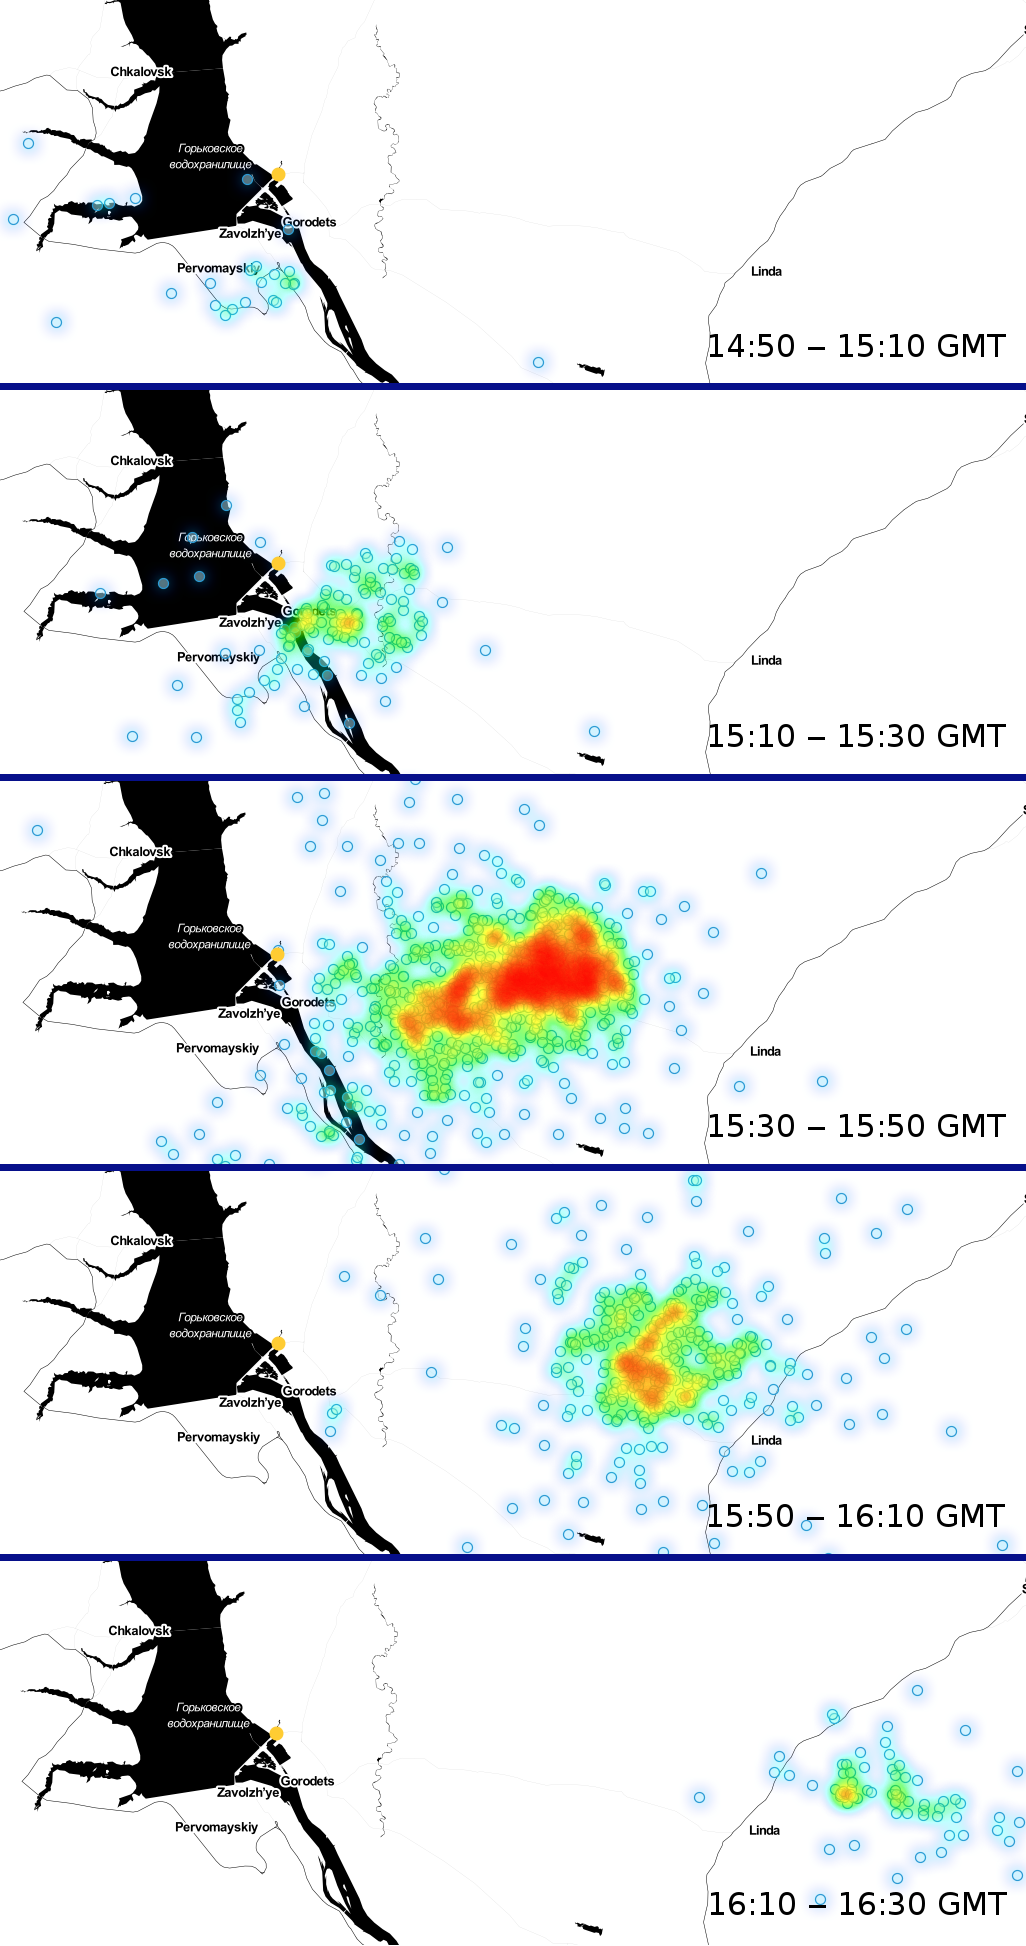
\includegraphics[width=0.45\linewidth]{lds-thunderstorm-move.png}}
	\caption{Визуализация грозы 16 июля 2016}
	\label{fig:lds-thunderstorm-move}
\end{figure}

На \figRef{fig:lds-thunderstorm-move} приведены показания ГПС во временных интервалах 20 мин. Кружками без заливки показаны отдельные молнии, цветом "--- плотность молний на единицу площади в относительных единицах. На \figRef{fig:lds-thunderstorm-freq} показана динамика развития грозы. По вертикали показано количество зарегистрированных молниевых разрядов в минуту. Учитываются как внутриоблачные, так и разряды типа облако-земля. На рисунках хорошо видно возникновение, развитие и угасание грозы.

Данная гроза унесла жизнь человека, купавшегося в Волге \cite{newsnn2016}. В точном соответствии с временем происшествия Нижегородская ГПС зарегистрировала несколько мощных разрядов типа облако-земля в воду вблизи места купания людей.

\begin{figure}[h]
	\center{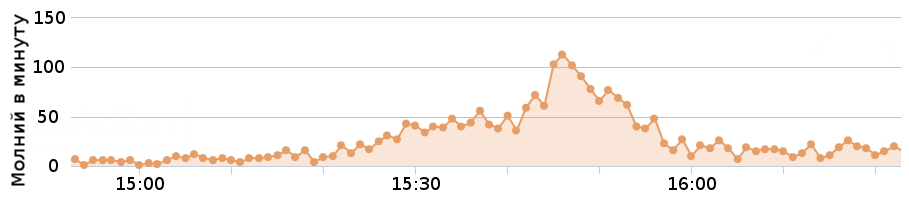
\includegraphics[width=\linewidth]{lds-thunderstorm-freq.png}}
	\caption{Динамика развития грозы 16 июля 2016. По вертикали приведено количество разрядов облако-облако и облако-земля в минуту, включая повторные компоненты}
	\label{fig:lds-thunderstorm-freq}
\end{figure}

\section{Валидация показаний ГПС}
\label{sec:lds-valid}
Важнейшей характеристикой любой грозопеленгационной системы является точность позиционирования разрядов. Этот показатель определяет применимость ГПС для решения тех или иных задач. Определение погрешности ГПС возможно непосредственным образом, либо "--- сравнением с другими системами определения положений молний.

Точные координаты и времена молниевых разрядов могут быть определены по информации, получаемой от молниеотводов, установленных на различных объектах, либо "--- от триггерных молний. Такой подход не применим в текущих условиях. На территории России нет полигонов, оборудованных устройствами для создания триггерных молний. Характерная частота разрядов облако-земля для средней полосы России составляет около 2~разрядов на квадратный километр в год \cite{BaruKononovSolomonic}, поэтому для сбора хотя бы сотни записей за конвективный сезон требуется не менее тысячи автоматических молниеотводов-регистраторов, распределенных по всей области покрытия ГПС.

Альтернативным способом валидации показаний ГПС является сравнение показаний с другими косвенными источниками информации о положении молний. В данной работе использованы данные международной системы WWLLN, а также показания допплеровского метеорадиолокатора (ДМРЛ) \cite{BulatovMiG}.

\begin{figure}[h]
	\center{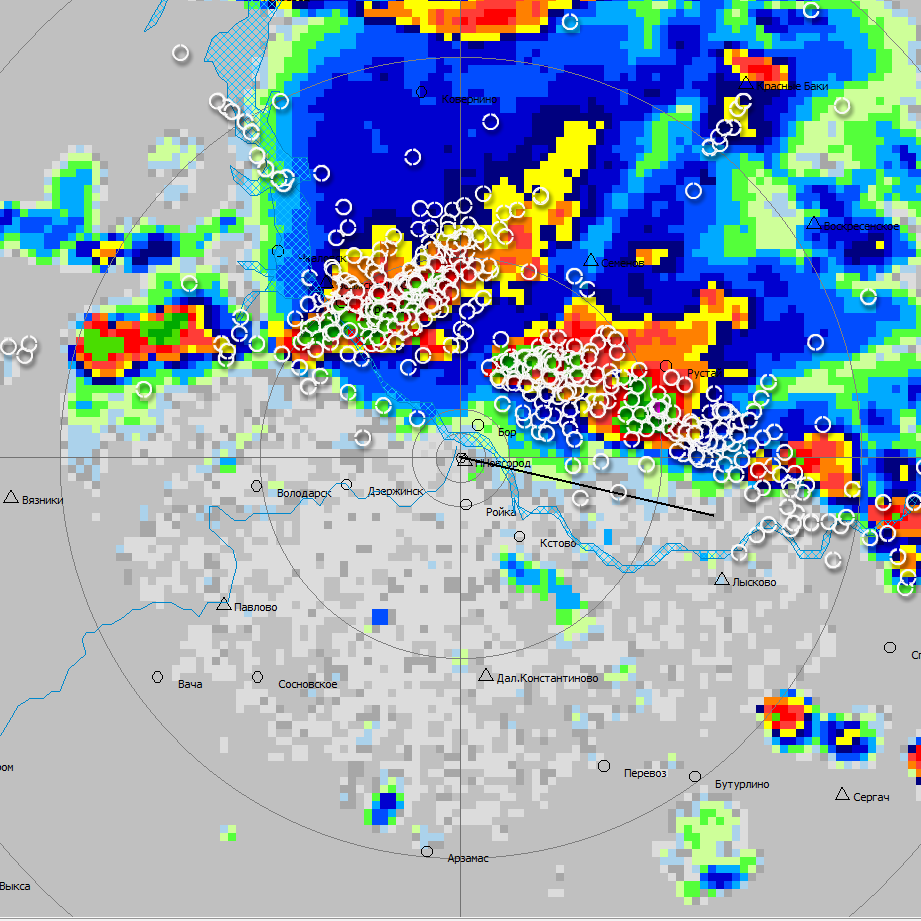
\includegraphics[width=\linewidth]{dmrl-lds.png}}
	\caption{Показания ГПС, наложенные на карту отражаемости ДМРЛ для грозы 5~июля 2015\,г. за промежуток 8:20$\ldots$8:30~GMT}
	\label{fig:dmrl-lds}
\end{figure}

Для качественной проверки точности грозопеленгационной системы проведено сравнение её показаний с данными ДМРЛ. На \figRef{fig:dmrl-lds} приведены отметки ГПС, наложенные на радиолокационную отражаемость облаков, полученную во время грозы 5~июля 2015\,г. за промежуток 8:20$\ldots$8:30~GMT. Наблюдается качественное согласование данных ДМРЛ и показаний системы. Аналогичная согласованность наблюдается для большинства интенсивных гроз конвективных сезонов 2014-2015\,гг. Проведение численного сравнения показаний не представляется возможным, поскольку между радиолокационной отражаемостью и наличием молний имеется лишь косвенная связь \cite{BulatovMiG}.

Точность глобальных систем грозопеленгации, покрывающих большие площади, может варьироваться в зависимости от расстояния до ближайших грозопеленгаторов. Международная глобальная грозопеленгационная система WWLLN покрывает территорию Европейской части России, однако разработчики системы не производили оценку точности её показаний на данной территории. Есть исследования, косвенными методами оценивающие точность WWLLN \cite{Gubenko2014}. В данной работе произведено непосредственное сравнение показаний нижегородской системы и WWLLN, что позволило получить оценки сверху на погрешности обеих систем в силу независимости их ошибок.

При сравнении показаний разработанной грозопеленгационной системы с показаниями следует WWLLN учитывать их особенности. 
Ближайшие грозопеленгаторы WWLLN расположены в Брянске (удаление от Нижнего Новгорода около~700 км), Соданкюле (Лапландия, ок.~1500 км), Ереване (ок.~1800 км) и Будапеште (ок.~2000 км). Грозопеленгаторы нижегородской системы на момент проведения исслдедования точности были расположены в Н. Новгороде, г. Городце и г. Семенове, образуя приблизительно равносторонний треугольник со стороной 60 км. Применение разных методов позиционирования разрядов, а также существенное пространственное удаление пеленгаторов двух систем друг от друга позволяют считать их ошибки независимыми случайными величинами.

\begin{table}[h]
	\begin{center}
		\begin{tabular}{l|l}
			Характеристика & Значение \\
			\hline
			Среднее отклонение по широте $\delta_{lat}$ & 1680\,м \\
			Среднее отклонение по долготе $\delta_{lon}$ & -1780\,м \\
			Стандартное отклонение по широте $\sigma_{lat}$ & 2700\,м \\
			Стандартное отклонение по долготе $\sigma_{lon}$ & 3080\,м \\
		\end{tabular}	
	\end{center}
	\caption{Различие показаний WWLLN и нижегородской ГПС}
	\label{tab:err-pars}
\end{table}

\begin{figure}[h]
	\center{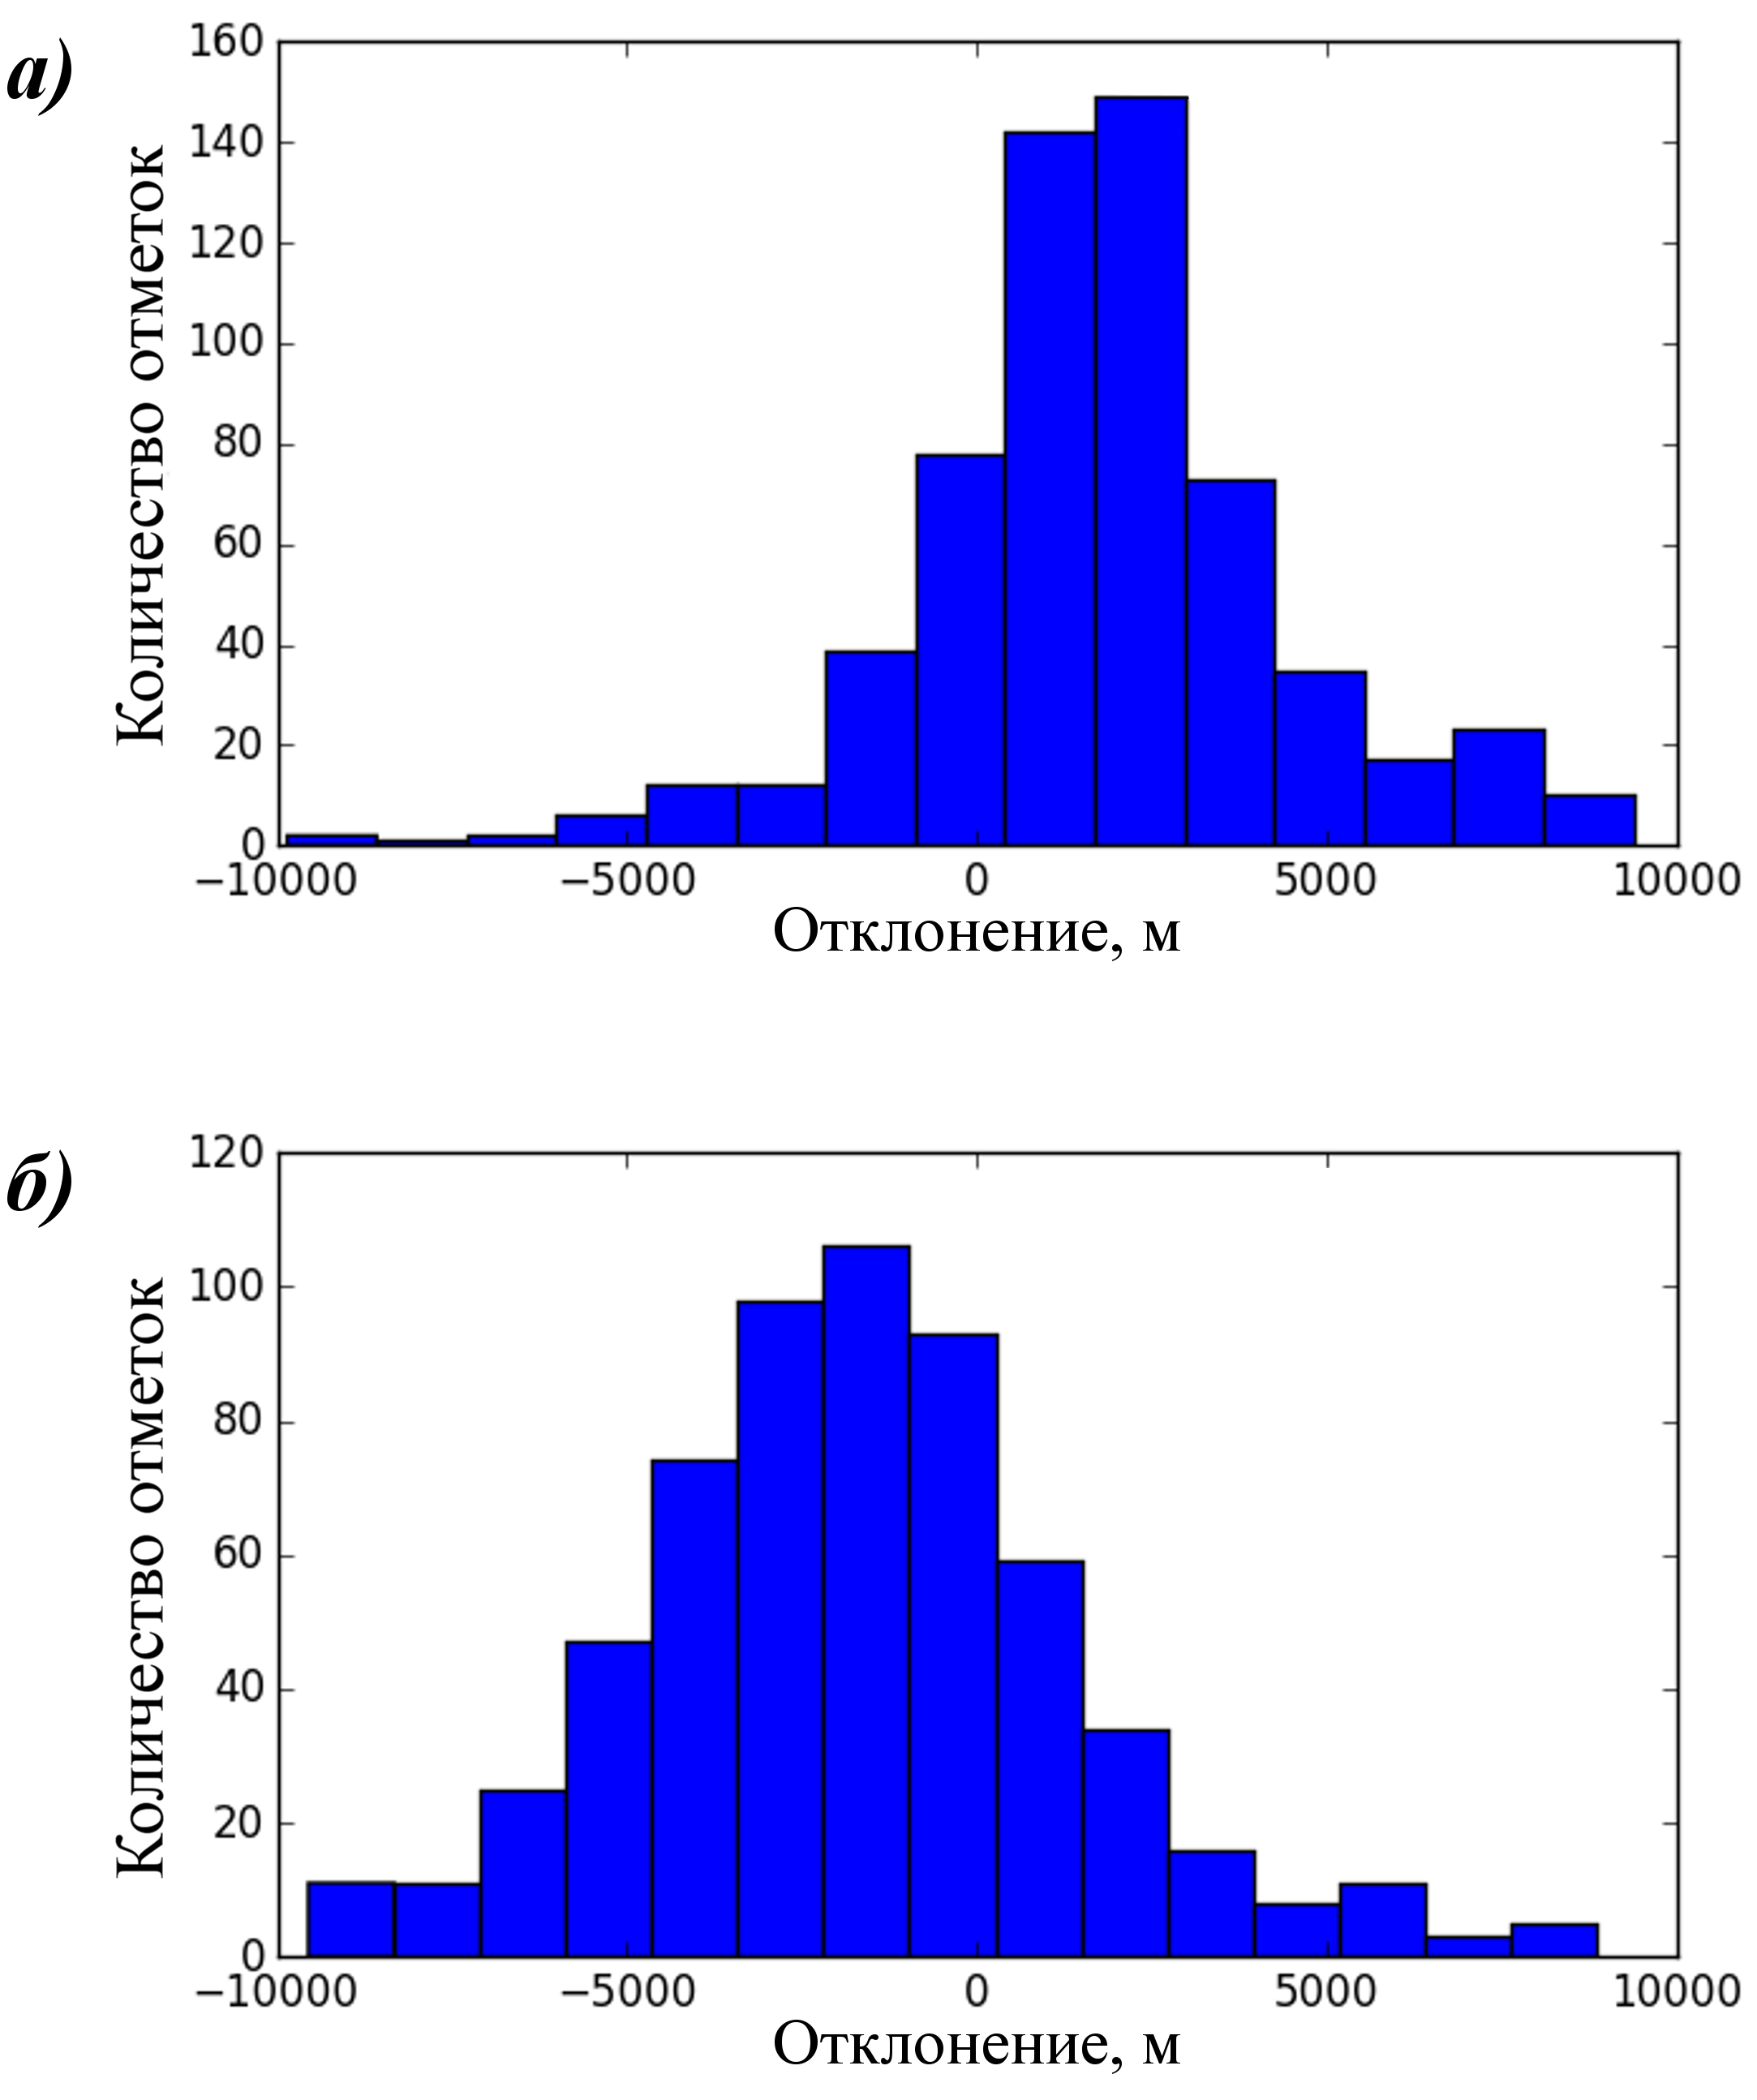
\includegraphics[width=0.5\linewidth]{lds-wwlln-diff.png}}
	\caption{Распределение различия показаний WWLLN и нижегородской ГПС по широте (а) и долготе (б)}
	\label{fig:lds-wwlln-diff}
\end{figure}

Обозначим ошибки WWLLN и нижегородской сети по широте и долготе соответственно за $\Delta_{lat}^{WWLLN}$, $\Delta_{lon}^{WWLLN}$, $\Delta_{lat}^{\text{Ниж}}$, $\Delta_{lon}^{\text{Ниж}}$. Обозначим различие показаний двух систем для одной и той же молниевой вспышки за $\Omega_{lat}$ и $\Omega_{lon}$ соответственно. Тогда, в силу независимости ошибок, для среднего значения $\delta_{lat}$, $\delta_{lon}$ и стандартного отклонения $\sigma_{lat}$, $\sigma_{lon}$ величин $\Omega_{lat}$ и $\Omega_{lon}$ справедливо:
\begin{equation}
	\begin{gathered}
		\delta_{lat, lon} = \overline{\Omega_{lat,lon}} = \overline {\Delta_{lat,lon}^{WWLLN}} + \overline {\Delta_{lat,lon}^{\text{Ниж}}}\\
		\sigma_{lat, lon} = \sigma(\Omega_{lat,lon}) = \sigma (\Delta_{lat,lon}^{WWLLN}) + \sigma (\Delta_{lat,lon}^{\text{Ниж}})
	\end{gathered}
\end{equation}
Таким образом, стандартное отклонение разности показаний может рассматриваться, как оценка сверху для стандартного отклонения ошибок каждой из систем на территории Нижегородской области.

Среди всех молниевых вспышек, отмеченных WWLLN за сезон 2014\,г., были выбраны точки, лежащие в области уверенного приёма нижегородской сети на расстоянии не более 150\,км от ближайшего пеленгатора. Затем отметкам молний WWLLN были поставлены в соответствие отметки, полученные нижегородской системой. Условием соответствия являлось 6различие моментов фиксации по времени не более, чем на $10^{-3}$\,с. Затем определялось различие положений отметок WWLLN и нижегородской сети по широте и долготе. После удаления выбросов, были определены параметры ошибок, приведённые в таблице \ref{tab:err-pars}. При этом было обработано 384 пар отметок WWLLN и нижегородской системы. На \figRef{fig:lds-wwlln-diff} приведены гистограммы отклонения значений нижегородской системы от WWLLN.

Величины  $\delta_{lat}$ и $\delta_{lon}$, вероятнее всего, объясняются систематической погрешностью WWLLN на территории Нижегородской области. Разностно-дальномерный метод, применяемый нижегородской системой, предварительная калибровка оборудования, а также симметрия исследуемой области относительно пеленгаторов исключают возникновение систематической ошибки по одной из координат. В то время как ближайшие приёмники WWLLN расположены в основном западнее исследуемой области, чем может быть объяснено соотношение между $\sigma_{lon}$ и $\sigma_{lat}$.

Таким образом, систематическая ошибка WWLLN на территории Нижегородской может быть оценена приблизительно, как 1780 м на юг и 1680 м на восток при стандартном отклонении 3 км. Стандартное отклонение нижегородской системы также может быть оценено сверху в 3 км. Данные величины могут быть уточнены в меньшую сторону в ходе дальнейших исследований.

\chapter{Исследование молниевой активности по данным ГПС}
Грозопеленгационные системы "--- эффективный инструмент исследования статистических характеристик молниевой активности. Основным вопросом климатологии молний является определение закономерностей поражаемости молниями территорий различных типов. В данной работе исследована зависимость количества гроз от рельефа и степени урбанизации местности. Показано наличие т.\,н. <<урбан-эффекта>> на территории Нижнего Новгорода. Выдвинута гипотеза об отрицательном влиянии мощных ТЭЦ на вероятность возникновения, либо прохождения грозы \cite{BulatovEnergetik2017}. 

По данным ГПС OpenLDS исследованы статистические характеристики повторных компонент обратных ударов на основе более, чем 1,5\,млн. зарегистрированных молний. Показано, что с ростом количества повторных компонент условная вероятность возникновения каждой следующей сначала увеличивается, а затем остаётся постоянной. Получена статистика временных интервалов между повторными компонентами молний, выявлены закономерности.

\section{Особенности распределения молний на территории Нижегородской области}
\label{sec:lds-distr}
Интенсивность молниевой активности на той или иной территории существенно зависит от различных факторов, таких, как тип и рельеф местности, удаленность от крупных водных ресурсов, интенсивность деятельности человека. Характеристиками, непосредственно влияющими на образование грозовых облаков и молний являются концентрация аэрозолей и аэроионов в воздухе, характерная температура и теплоемкость местности, средняя влажность, ветровые характеристики. Одним из проявлений неоднородности распределения молний является т. н. урбан-эффект: согласно некоторым исследованиям, молниевая активность над крупными городами существенно выше, чем над неурбанизированной местностью \cite{Farias2009,Farias2014,Pinto2004}. В работе \cite{BulatovMiG} подтверждено наличие урбан-эффекта на территории Нижнего Новгорода по сравнению с другими участками области.

Для определения интенсивности молниевой активности возможно применение различных показателей: общее количество молниевых разрядов, количество разрядов облако-земля, количество гроз в течение конвективного сезона, суммарный заряд, переносимый молниями в землю и т.п. В работе \cite{BulatovMiG} в качестве основного параметра рассматривается общее количество молниевых разрядов на единицу площади. Такой параметр характеризует грозоопасность местности. Однако важное значение для хозяйственной деятельности и эксплуатации энергетических систем также имеет общее количество гроз в течение конвективного сезона.

В данной работе грозопеленгационной определено системы для количество нескольких гроз участков по данным местности нижегородской на территории Нижегородской области. Под грозой понимается молниевая активность не менее чем 10 разрядов в минуту в радиусе 5 км от опорной точки. Две грозы считаются различными, если в промежутке между ними как минимум в течение часа не зарегистрировано ни одной молнии над исследуемой областью. В качестве опорных точек выбраны следующие:
\begin{enumerate}
	\item Нижний Новгород (56.327\textdegree\,с.\,ш.; 44.003\textdegree\,в.\,д.) "--- мегаполис с населением 1,2~млн.~человек.
	\item Ковернино (57.125\textdegree\,с.\,ш.; 43.812\textdegree\,в.\,д.) "--- поселок городского типа с населением ок.
	7000 человек, сельская местность. Не более 50\% окрестной территории занято	лесом, остальное "--- сельскохозяйственные угодия, вырубки, пастбища и молодые посадки леса.
	\item Керженский биосферный заповедник (56.548\textdegree\,с.\,ш.; 44.923\textdegree\,в.\,д.) "--- практически
	сплошной лес, урбанизация отсутствует.
	\item Заволжье (56.645\textdegree\,с.\,ш.; 43.392\textdegree\,в.\,д.) "--- город на берегу Горьковского водохранилища в непосредственной близости от г.~Городец. Суммарная численность населения обоих городов около 70~тыс.~человек. На территории г.~Заволжье находится обширная инфраструктура Нижегородской ГЭС, состоящая из открытых электрораспределительных устройств, в том числе для ЛЭП напряжением 220 кВ и 110 кВ.
	\item Балахна (56.480\textdegree\,с.\,ш.; 43.540\textdegree\,в.\,д.) "--- город на правом берегу Волги с численностью населения 50~тыс.~человек. В Балахне находится Нижегородская ГРЭС им. А.\,В.~Винтера с установленной электрической мощностью 144\,МВт и тепловой 566\,Гкал/час.
	\item Кстово (56.151\textdegree\,с.\,ш.; 44,195\textdegree\,в.\,д.) "--- город с населением 67~тыс.~человек. В Кстово
	располагается Новогорьковская ТЭЦ с установленной электрической мощностью
	548,3 МВт и тепловой 626 Гкал/час.
\end{enumerate}

Помимо прочих факторов, выбранные области позволяют исследовать влияние объектов энергетической инфраструктуры на вероятность возникновения гроз.

\begin{figure}[h]
	\center{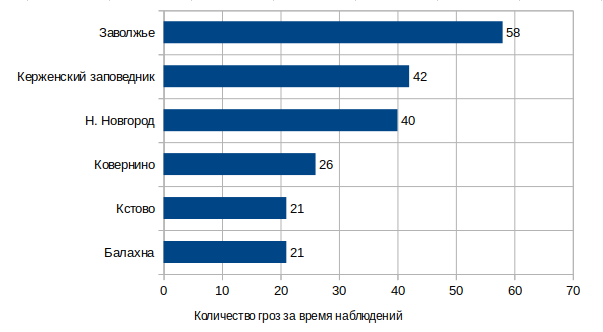
\includegraphics[width=0.8\linewidth]{lds-places-stat.png}}
	\caption{Количество гроз над исследуемыми территориями, зарегистрированных за период с июля 2014\,г. по август 2016\,г.}
	\label{fig:lds-places-stat}
\end{figure}

Для данных участков за промежуток с июля 2014\,г. по август 2016\,г. определено суммарное количество гроз. Результаты приведены на \figRef{fig:lds-places-stat}. Только около 15\% гроз покрывали одновременно все исследуемые территории, в большинстве случаев они имели более локальный характер. В целом, для исследованных регионов характерна существенная неоднородность вероятности прохождения гроз с различием для отдельных областей более, чем в 2,7~раза, что говорит о наличии существенных механизмов, влияющих на грозовую активность.

Для объяснения существенного различия в количестве гроз были предложены некоторые гипотезы. Из диаграммы видно, что наибольшее количество гроз характерно для г.~Заволжье. В качестве возможного объяснения высоких показателей можно привести сочетание двух факторов: нахождение на берегу водохранилища и большая площадь электроэнергетической инфраструктуры.

Минимальное количество гроз зарегистрировано в окрестностях городов Балахна и Кстово. В отличие от остальных исследуемых территорий, в обоих городах находятся мощные ТЭЦ. Детальное рассмотрение структуры отдельных гроз в окрестностях Балахны и Кстово средствами нижегородской ГПС также показало, что грозы средней и малой относительной интенсивности как бы огибают данные участки. Заметим, что на ГРЭС в Балахне для охлаждения используется пруд значительной площади, а на Новогорьковской ТЭЦ в Кстово для охлаждения используются градирни Это позволяет выдвинуть гипотезу о влиянии инфраструктуры ТЭЦ на снижение частоты гроз в окрестности. Такой эффект может объясняться большим локальным выбросом тепла, влияющим на развитие грозовых облаков, а также поступлением водяного пара от охлаждающих систем и образующегося в результате сгорания топлива одновременно с образованием углекислого газа. Изучение конкретного механизма воздействия выходит за рамки данной работы и является задачей дальнейших тематических исследований.

В окрестностях Ковернино вероятность гроз также не высока, однако на 23\% превышает такой показатель для Кстово и Балахны. При этом для Ковернино картина в целом совпадает со всем Ковернинским районом, никак не выделяя районный центр, что не справедливо для Кстово и Балахны. Поэтому логичным объяснением снижения частоты гроз может являться отсутствие промышленности, низкая численность населения и относительно малое количество леса.

Другим интересным результатом является приблизительно одинаковый уровень грозовой активности для двух совершенно разных типов местности, удаленных на расстояние порядка 65 км: города-мегаполиса Н. Новгорода и Керженского биосферного заповедника. В обоих случаях наблюдается высокая вероятность гроз, что обусловлено различными факторами. В мегаполисе возможной причиной может являться большое количество аэрозолей, что согласуется с аэрозольной теорией урбан-эффекта \cite{Farias2009}. В случае леса причиной может быть повышенная интенсивность образования аэроионов, отличия в суточном цикле влажности и другие факторы.

\section{Статистические характеристики повторных разрядов}
\label{sec:lds-stat-rep}
Хорошо известно, что главная стадия молнии, <<обратный удар>>, может многократно повторяться. Считается, что примерно половина всех разрядов облако-земля является многократными, причём количество повторений в отдельных случаях может достигать десятков раз \cite{RakovUman2005}. 

Для исследования мультипликативности обратного удара применимы региональные грозопеленгационные системы. В отличие от глобальных, они регистрируют практически 100\% молниевых вспышек в определенной местности. При достаточном временном разрешения такие системы хорошо различают компоненты обратного удара. ГПС~OpenLDS, разработанная в рамках данной работы, позволила исследовать статистические характеристики повторных разрядов на территории Нижегородской и соседних областей.

Для анализа использованы все данные, полученные системой за время функционирования с 2014 по 2017\,гг. За данный период грозопеленгационная система зарегистрировала более~2,2~млн.~молниевых разрядов.

\subsection{Определение повторных компонент молний}
Временное разрешение ГПС OpenLDS позволяет разрешать повторные компоненты молний. Информация, предоставляемая ГПС, представляет собой координаты, широту и долготу~$(\theta_i, \varphi_i)$ и время~$t_i$ для каждого разряда. Условием того, что два последовательно зарегистрированных разряда являются компонентами одной молнии, является их географическая близость и достаточно малый промежуток времени между ними. Однако, если промежуток времени слишком мал, это может означать, что ГПС зарегистрировала дважды один и тот же разряд. Таким образом, условием того, что разряд $i+1$ является повтором после разряда $i$ является:
\begin{equation}
	\begin{gathered}
		\rho\left[(\theta_i, \varphi_i), (\theta_{i+1}, \varphi_{i+1})\right] < \rho_{max},\\ \Delta t_{min} < t_{i+1} - t_i < \Delta t_{max}
		\label{eq:criteria}
	\end{gathered}
\end{equation}
где функция $\rho$ "--- расстояние между точками на поверхности Земли.

В качестве величины $\rho_{max}$ в формуле \eqref{eq:criteria} взята погрешность ГПС, 3\,км. В качестве величины $\Delta t_{max}$ "--- максимальной задержки между повторными компонентами, взято 0,4\,с. Такое значение гарантировано превышает средний интервал между компонентами обратного удара \cite{RakovUman2005}. Величина $\Delta t_{min} = 100$\,мкс, что превышает характерную длительность тока обратного удара. Экспериментально установлено, что для величины $\Delta t_{min} \in [5\text{\,мкс}, 500\text{\,мкс}]$ результаты статистической обработки данных не меняются, что позволяет сделать вывод о практически полном отсутствии случаев двойной регистрации однократного обратного удара с интервалом более 5\,мкс.

Рассмотрим надёжность данного критерия с точки зрения ложноположительного результата. Теоретически, возможно возникновение двух независимых молний на расстоянии, меньшем $\rho_{max}$ через промежуток времени, меньший $\Delta t_{max}$. Однако, по данным ГПС, самые сильные грозы в регионе имеют интенсивность не более 250 разрядов в минуту считая все компоненты и внутриоблачные разряды. Оценивая снизу область такой грозы в $1000\,\text{км}^2$, получаем вероятность ложноположительного обнаружения повторной компоненты~$P_{err}=0,5\%$. Данная оценка справедлива всего для нескольких грозовых часов в году и становится существенно меньше для менее интенсивных гроз. Что касается N-кратных разрядов, вероятность ложноположительного их детектирования равна $P_{err}^N$, что представляет собой исчезающе малую величину для выборки в 2,2~млн~записей.

Особенностью грозопеленгационной системы OpenLDS, на данный момент, является невозможность надёжного различения типа и знака молниевого разряда. Однако, считается, что количество повторных компонент главной стадии молнии более 3 преимущественно характерно для отрицательных разрядов типа облако-земля \cite{RakovUman2005}. Таким образом, основные выводы работы справедливы для отрицательных молний, ударяющих в землю.

\begin{figure}[h]
	\center{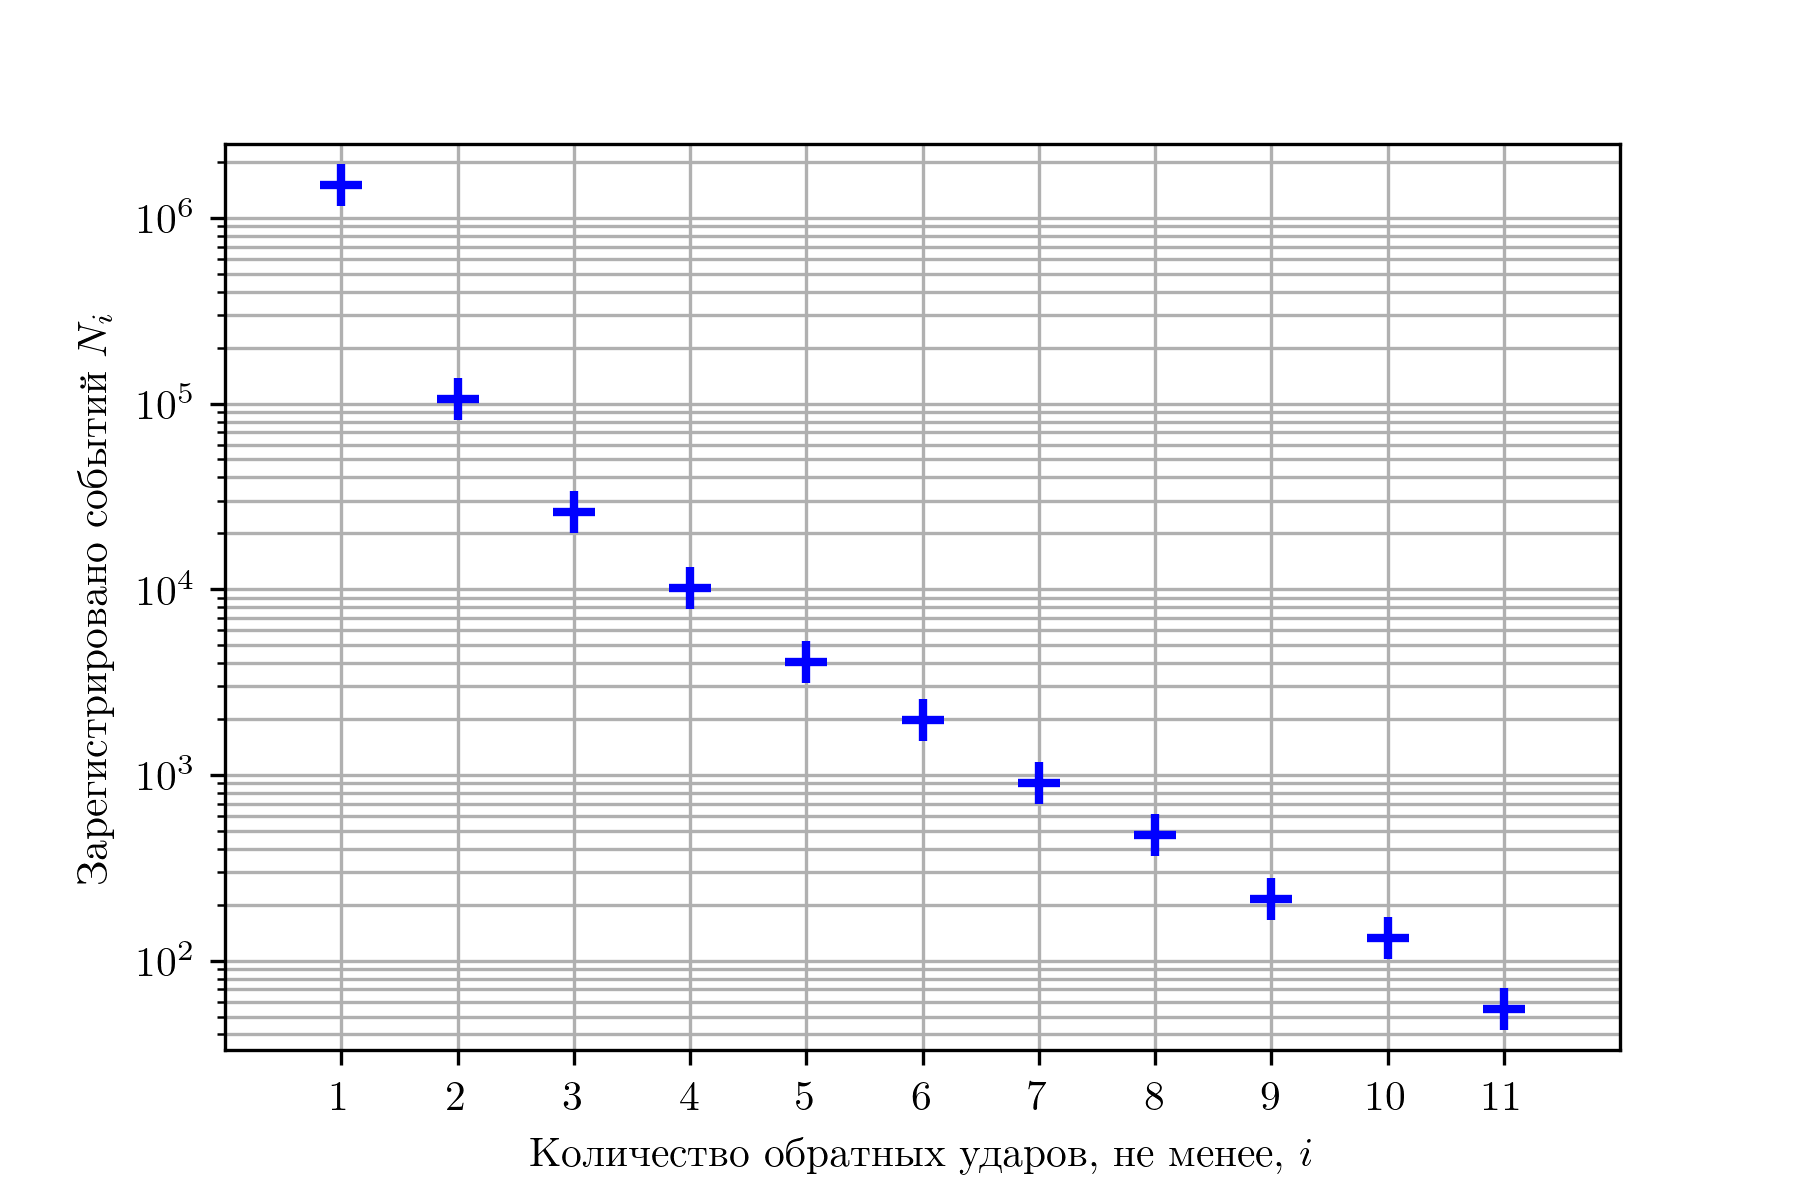
\includegraphics[width=0.9\linewidth]{lds-reps.png}}
	\caption{Количество событий с определенным числом повторов обратного удара}
	\label{fig:lds-reps}
\end{figure}

\subsection{Повторяемость обратного удара}
За время наблюдений зарегистрировано приблизительно 1,5\,млн. молний, 106\,тыс. из которых имели повторные компоненты. В области покрытия ГПС за время наблюдения зарегистрировано до 16 повторов главной компоненты молнии, наблюдалось 3 таких события во время интенсивных гроз в августе 2016\,г.

Рассмотрим статистику количества повторов главной стадии молнии, полученную на основе критерия \eqref{eq:criteria}. На \figRef{fig:lds-reps} приведена зависимость количества зарегистрированых событий $N_i$ от числа повторов обратного удара $i$ в полу-логарифмическом масштабе. Величина $N_i$ включает в себя как случаи, когда обратный удар повторился ровно $i$ раз, так и случаи с $i+1$, $i+2$, $...$ повторениями. Численные значения величины $N_i$ приведены в таблице \ref{tab:lds-intervals}.

\begin{figure}[h]
	\center{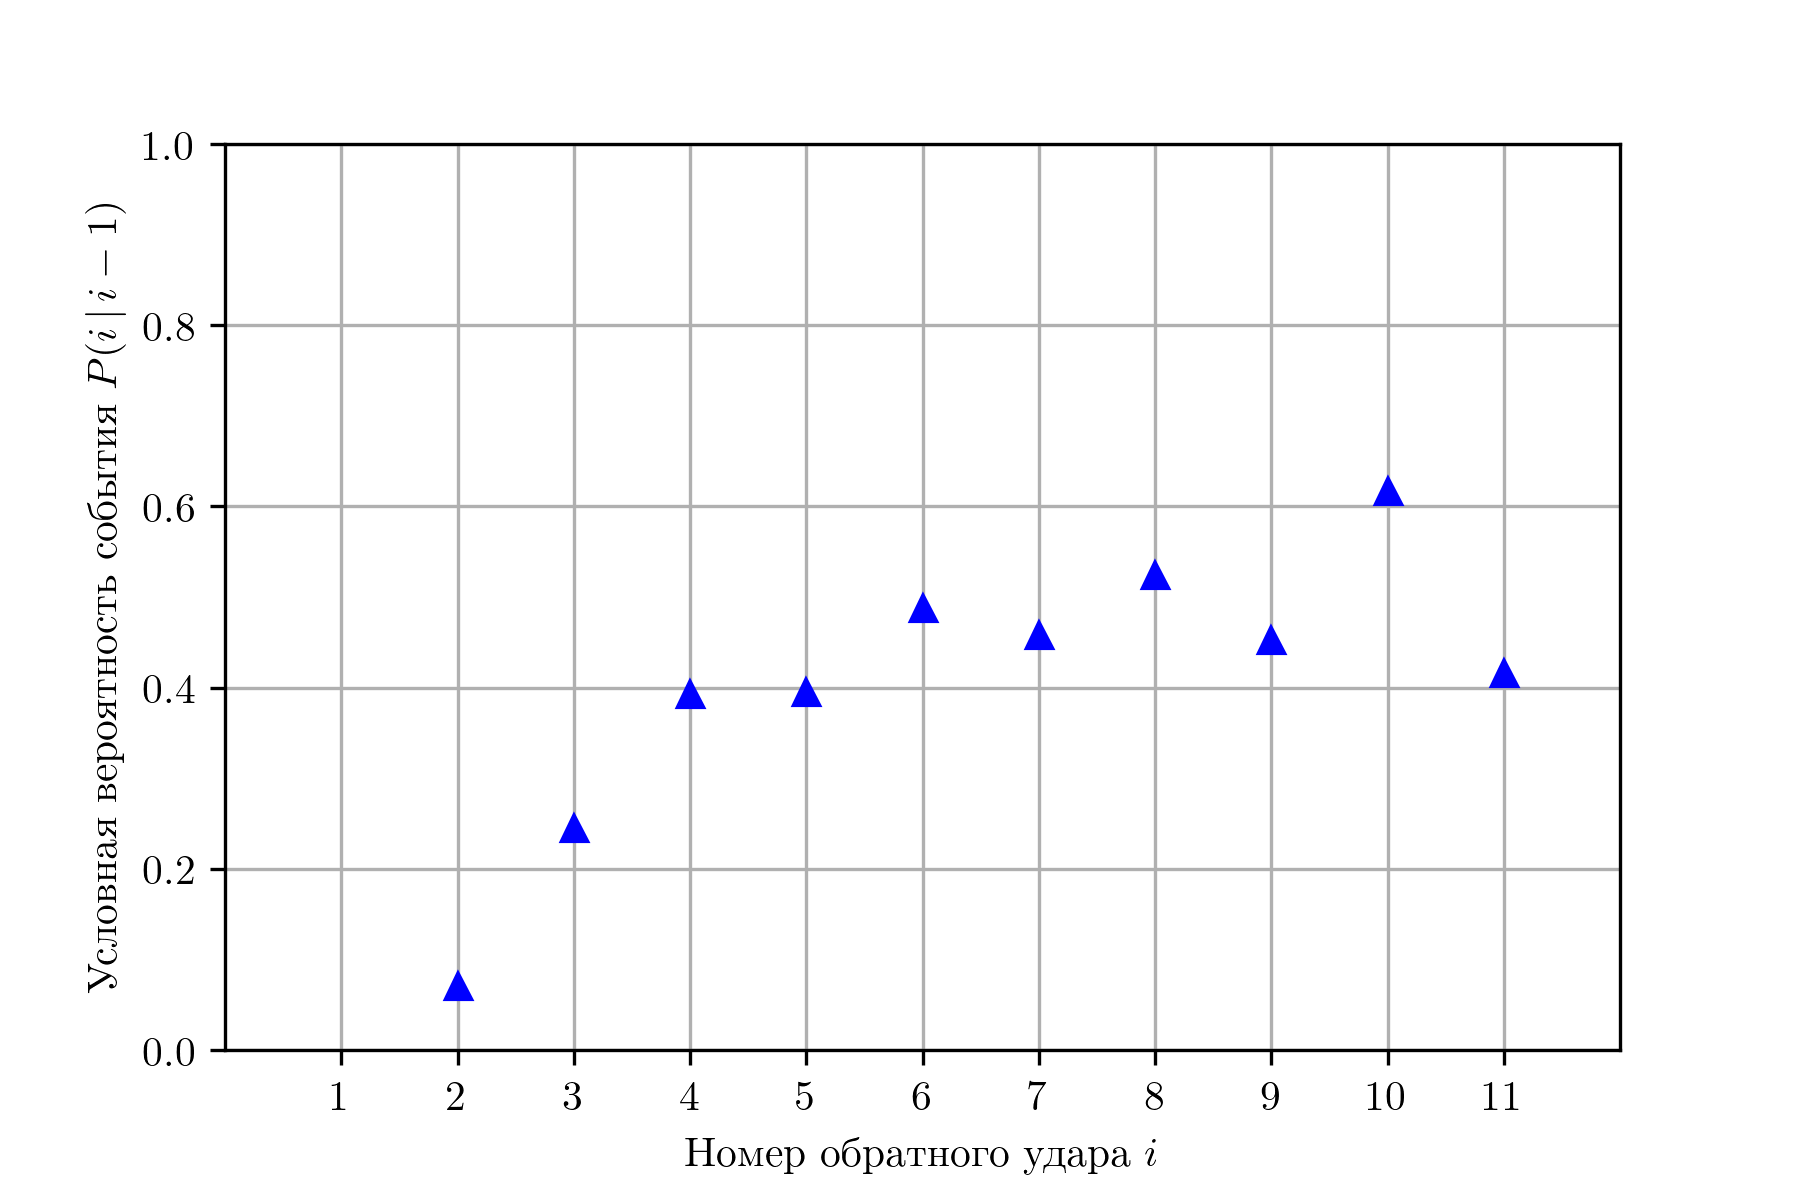
\includegraphics[width=0.9\linewidth]{lds-probs.png}}
	\caption{Условные вероятности возникновения повторных обратных ударов}
	\label{fig:lds-probs}
\end{figure}

Если провести кривую через точки на \figRef{fig:lds-reps}, будет заметна выпуклость кривой вниз. Рассмотрим условную вероятность развития $i$-го повтора обратного удара при условии того, что повтор $i-1$ имел место:
\begin{equation}
	P(i\,|\,i-1) = \frac{N_i}{N_{i-1}}.
\end{equation}
Другими словами, если мы наблюдаем за грозой сразу после того момента, когда произошло $i$ повторов главной стадии молнии, с вроятностью $P(i\,|\,i-1)$ произойдёт и $(i+1)$-ый повтор.

На \figRef{fig:lds-probs} приведена зависимость величины $P(i\,|\,i-1)$ от $i$. Её численные значения приведены в таблице \ref{tab:lds-intervals}. Условная вероятность существенно растёт от 0,24 до 0.52 на интервале от 2 до 8 повторов обратного удара. Далее вероятность достигает насыщения и её колебания обуславливаются уменьшением мощности выборки. 

\subsection{Статистика временных интервалов}

Рассмотрим временные интервалы между компонентами одной молнии. На \figRef{fig:lds-hist} приведены гистограммы интервалов между первым (главным) и вторым обратными ударами, между вторым и третьим, третьем и четвёртым, четвертым и пятым. Распределения нормированы на единицу, графики представляют собой плотности вероятности. В таблице~\ref{tab:lds-intervals} приведены численные значения средних ($\overline {\Delta t_i}$) и медианных ($\Delta t_i^m$) интервалов между разрядами, а также их стандартного отклонения. Эти же данные представлены на графике на \figRef{fig:lds-graph}.

\begin{figure}[h]
	\center{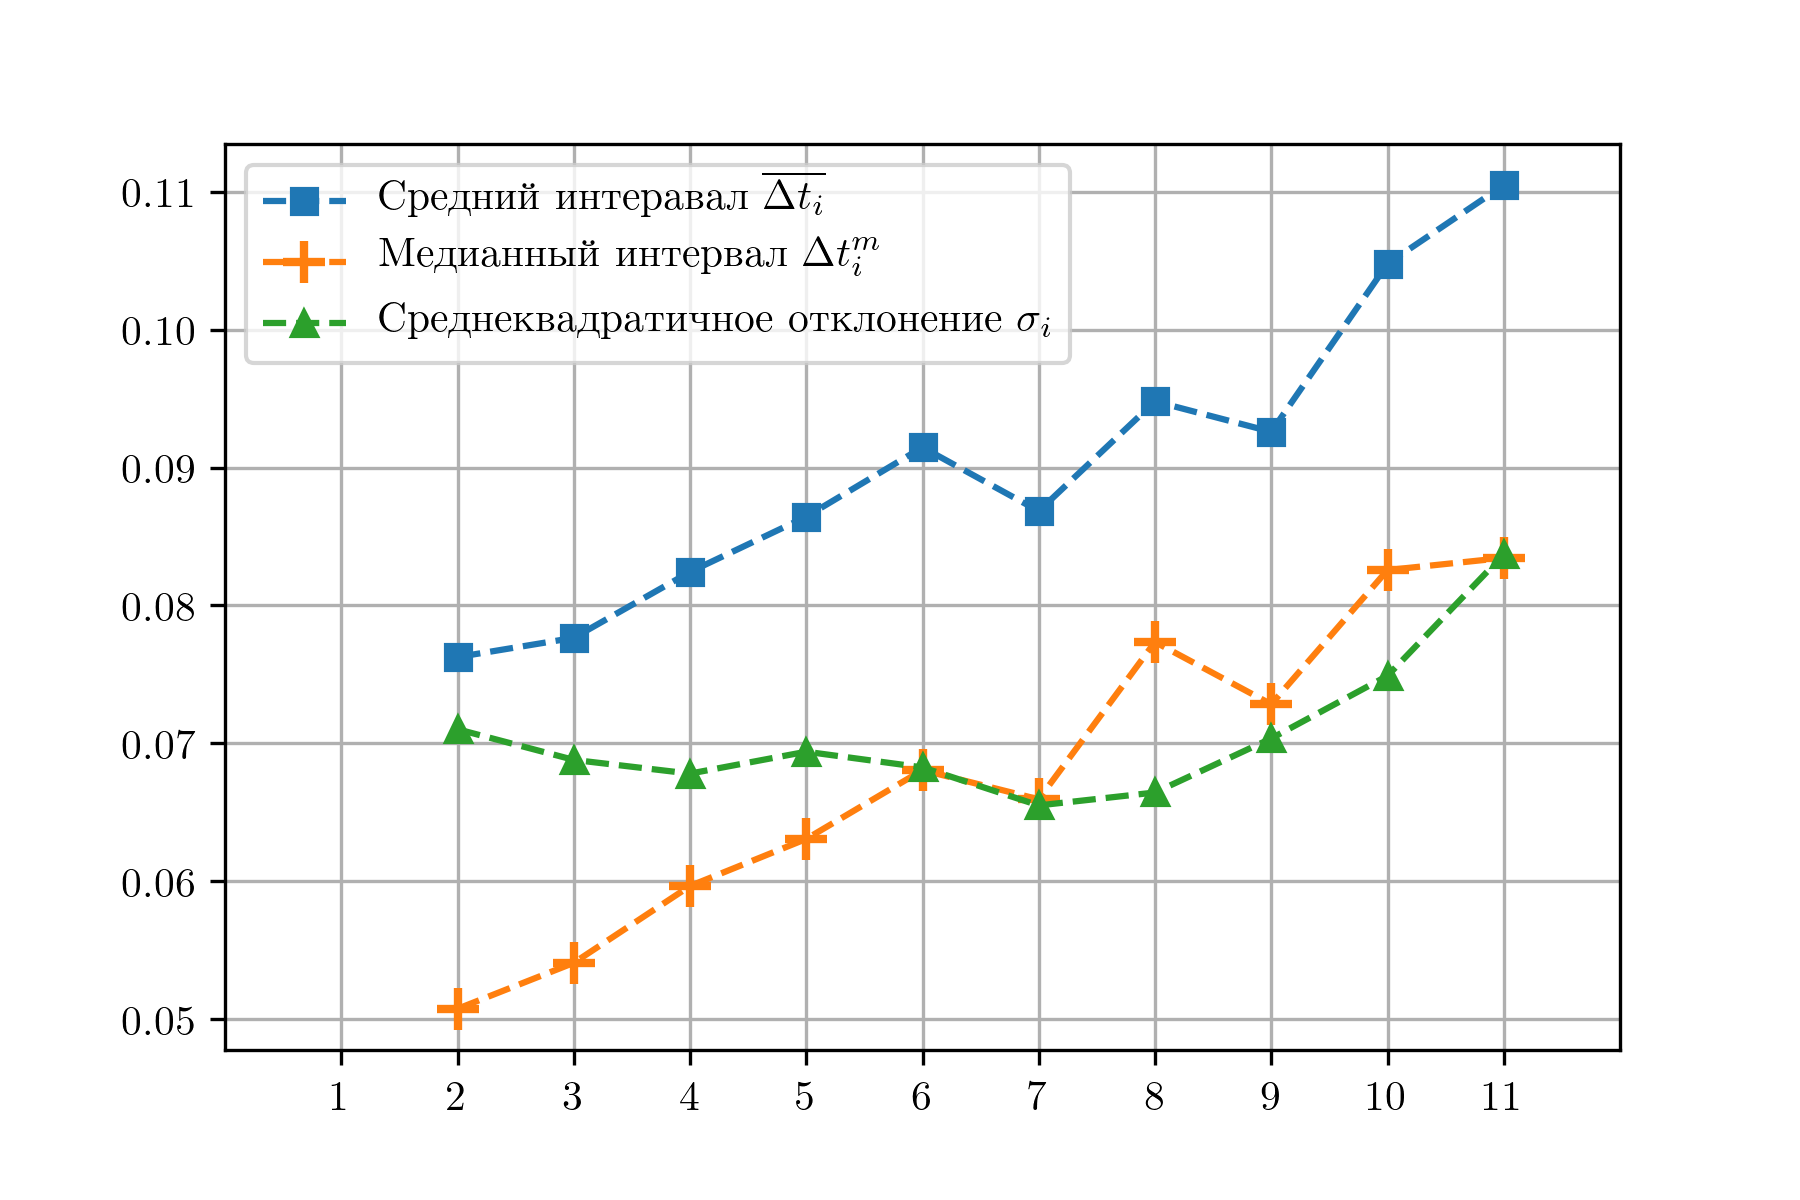
\includegraphics[width=0.9\linewidth]{lds-graphs.png}}
	\caption{Зависимость среднего, медианного значений временного интервала и его стандартного отклонения от номера повтора компоненты разряда}
	\label{fig:lds-graph}
\end{figure}

\begin{table}[h]
	\centering
	\begin{tabular}{ c | c | c | c | c | c }
		%\hline
		
		\begin{sideways} Количество обратных ударов $i$ \end{sideways} &
		\begin{sideways} Количество событий $N_i$ \end{sideways} &
		\begin{sideways} Условная вероятность $P(i\,|\,i-1)$ \end{sideways} &
		\begin{sideways} Средний интервал $\overline {\Delta t_i}$, мс \end{sideways} &
		\begin{sideways} Медианный интервал $\Delta t_i^m$, мс \end{sideways} &
		\begin{sideways} Стандартное отклонение $\sigma_i$, мс \end{sideways} \\ \hline
		\rule{0pt}{14pt} 1 & 1394457 & -- & -- & -- & -- \\
		\rule{0pt}{14pt} 2 & 80280 & 0.07 & 76 & 50 & 71 \\
		\rule{0pt}{14pt} 3 & 15765 & 0.24 & 77 & 54 & 69 \\
		\rule{0pt}{14pt} 4 & 6180  & 0.39 & 82 & 60 & 68 \\
		\rule{0pt}{14pt} 5 & 2065  & 0.40 & 86 & 63 & 69 \\
		\rule{0pt}{14pt} 6 & 1068  & 0.49 & 91 & 68 & 68 \\ 
		\rule{0pt}{14pt} 7 & 429   & 0.46 & 87 & 66 & 65 \\ 
		\rule{0pt}{14pt} 8 & 259   & 0.52 & 95 & 77 & 66 \\ 
		\rule{0pt}{14pt} 9 & 82    & 0.45 & 93 & 73 & 70 \\ 
		\rule{0pt}{14pt} 10 & 77   & 0.61 & 105 & 83 & 74 \\ 
		\rule{0pt}{14pt} 11 & 19   & 0.41 & 110 & 83 & 83 \\ 
	\end{tabular}
	\caption{Статистические характеристики интервалов между повторными разрядами}
	\label{tab:lds-intervals}
\end{table}

\subsection{Обсуждение результатов}
Рост и насыщение величины $P(i\,|\,i-1)$ имеет существенное значение и является одним из главных результатов исследования (см. \figRef{fig:lds-probs}). Рассмотрим факторы, которые могут прервать последовательность повторений обратного удара для среднестатистической отрицательной молнии: деградацию молниевого канала и истощение заряда облака.

Известно, что при наличии повторных компонент большая часть молниевого канала <<переиспользуется>> этими компонентами \cite{Rakov-PhysicsOfLightning}. В промежутках между вспышками канал может деградировать: остывать, рекомбинировать и разрушаться под действием порывов ветра и других факторов. Процесс деградации происходит по определенным законам и время разрушения канала зависит от его начальных характеристик. После прохождения разряда канал <<обновляется>>, и процесс распада начинается заново. При распаде канала до некоторого критического состояния дальнейшее повторение обратных ударов становится невозможным.

%<<Качество канала>> определяется, в первую очередь, температурой нейтрального газа и остаточной ионизацией, а также пространственным распределением этих параметров. Однако, для упрощения, <<качество>> можно параметризовать в виде некоторой переменной $Q$. Тогда, вероятность развития повторной компоненты определяется величиной $Q$ и доступностью необходимого для стреловидного лидера заряда. С течением времени происходит уменьшение величины $Q(t+\Delta t) = Q(t)\cdot \exp(-\alpha t)$. С каждым разрядом~$Q$ мгновенно увеличивается на некоторую величину $\Delta Q$. Если интервал между разрядами составляет $\Delta е$, то в зависимости от соотношения $\alpha$, $\Delta Q$ и $\Delta t$ среднее значение качества канала может как падать, так и расти.

Другим фактором, влияющим на возможность развития разряда, являться истощение заряда в досягаемой части облака. Транспортная система, собирающая заряд, имеет ограниченные возможности прорастания вглубь облака и конечную скорость сбора нового заряда. Количество доступного заряда может быть в принципе ограниченным.

Согласно экспериментальным данным, полученным в рамках исследования, показано, что средний интервал $\overline {\Delta t_i}$ между повторными компонентами монотонно увеличивается от 76 до 110\,мс (\figRef{fig:lds-graph}). Это подтверждает замедление процесса сбора заряда. Однако, если бы доступный для среднестатистической молнии заряд мог бы быть исчерпан одной многокомпонентной молнией, наблюдалось бы уменьшение условной вероятности развития новой компоненты начиная с некоторого характерного числа повторов. Другими словами, одна многокомпонентная молния не способна разрядить облако на масштабах её транспортной системы.

<<Качество канала>> определяется, в первую очередь, температурой нейтрального газа и остаточной ионизацией, а также пространственным распределением этих параметров. В рамках данного подхода, рост и насыщение величины $P(i\,|\,i-1)$ объясняется следующим образом: когда средний интервал между молниями $\overline {\Delta t_i}$ мал, каждая следующая компонента дополнительно прогревает канал и генерирует ионы. Этот эффект накапливается и повышает вероятность последующих компонент. Однако, когда $\overline {\Delta t_i}$ увеличивается из-за растущих трудностей при сборе заряда, растёт также и время деградации канала между разрядами, и процесс деградации уравновешивает нагрев и ионизацию при разрядах. В дальнейшем, с ростом $i$, деградация начнёт доминировать и условная вероятность будет снижаться. Однако такой эффект не наблюдается при значениях $i \le 12$.

\begin{figure}[h]
	\center{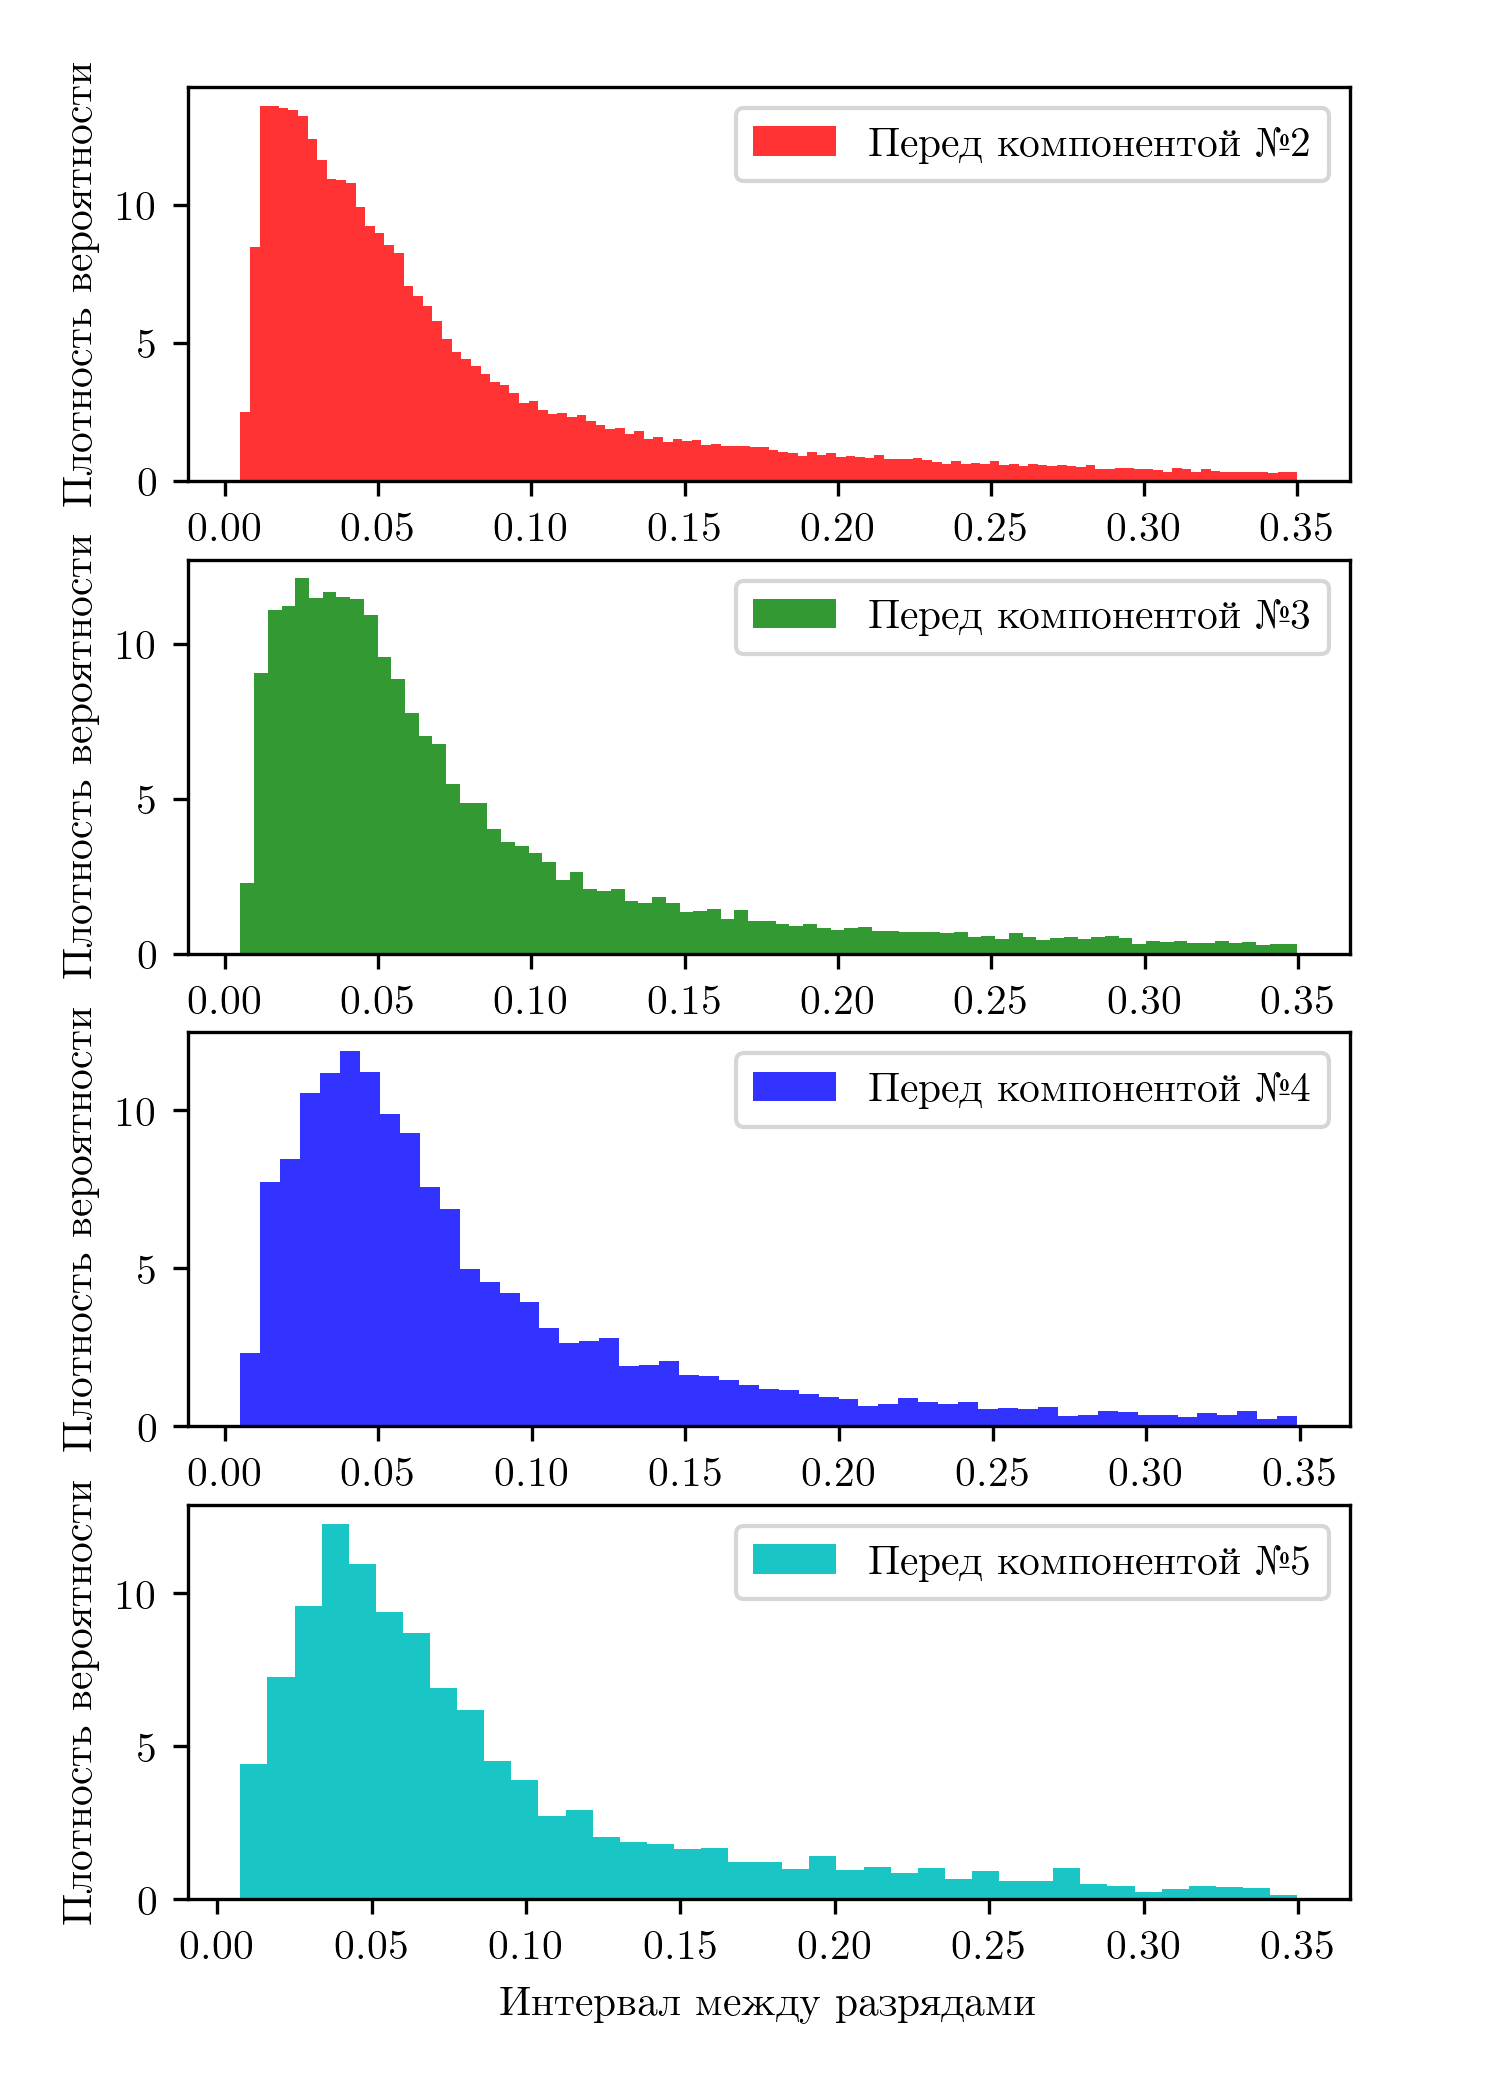
\includegraphics[width=0.8\linewidth]{lds-hist.png}}
	\caption{Распределение временных интервалов перед повторными обратными ударами}
	\label{fig:lds-hist}
\end{figure}

\section{Выводы}
Автором разработана и введена в эксплуатацию региональная грозопеленгационная система OpenLDS. ГПС функционирует с 2014\,г., и по данным на 2017\,г. покрывает территорию диаметром~1500\,км. За время работы системы зарегистрировано более 1,5\,млн. как однокомпонентных, так и многокомпонентных молний.

Проведено исследование точности ГПС OpenLDS на основе сравнения её показаний с данными ДМРЛ и WWLLN. Погрешность позиционирования молний системой OpenLDS оценена сверху величиной 3\,км. Также, оценена погрешность WWLLN на территории Нижегородской области.

На основе данных, полученных ГПС, исследована поражаемость молниями территорий различных типов. Предложена гипотеза отрицательного влияния ТЭЦ на количество гроз в непосредственной близости. 

Исследованы особенности статистики повторных компонент молниевых разрядов. Показано, что условная вероятность каждой следующей компоненты растёт и входит в насыщение с ростом количества компонент. Показано, что средний интервал между повторными компонентами растёт. Предложено объяснение данных закономерностей.



\FloatBarrier
